% globale Parameter (Papierformat, Schriftgroeße, Trennlinien, Doppelseitig)
\documentclass[a4paper, 11pt, headsepline,footsepline,twoside,abstract]{scrbook}


%%% Verwendete Pakete %%%

\usepackage{url}
\usepackage{geometry} % Seitenraender
\usepackage{fancyhdr} % Schoenere Kopf/Fußzeilen
\usepackage[utf8]{inputenc} % Kodierung
\usepackage[ngerman]{babel} % Sprache
\usepackage{graphicx}  % Bildchen
\usepackage{float}  % Bildchen2
\usepackage{setspace} % fuer Zeilenabstand
\usepackage[T1]{fontenc} % fuer Schriftart
%\usepackage{cite} % fuer Zitate
\usepackage[numbers,square]{natbib} % Package für Zitierstil
\usepackage{pgfplots} % Plots
\usepackage[justification=RaggedRight, singlelinecheck=false, margin=1.5cm]{caption}  % huebschere Captions
\usepackage[version=3]{mhchem} % chemische Formeln
\usepackage{booktabs} % schoenere Tabellen
\usepackage{multirow} % s.o.
\usepackage{ifthen} % s.o.
\usepackage{subfigure} % Grafiken nebeneinander darstellen
\usepackage{textcomp} %Euro-Zeichen
\usepackage{siunitx} % Einheiten korrekt anzeigen
%\sisetup{
% locale = DE ,
% per-mode = symbol,
% separate-uncertainty %+- Notation
%}
%\DeclareSIUnit{\masspercent}{m\%}
%\newcommand{\euro}{\,\texteuro\ } %Euro einfuegen

%Schriftart aendern
\newcommand{\changefont}[3]{
\fontfamily{#1} \fontseries{#2} \fontshape{#3} \selectfont}
\changefont{ptm}{m}{n}

% Zeilenabstand 1,5
\onehalfspacing

% weniger breite Seitenraender
\geometry{a4paper,left=28mm,right=28mm, top=32mm, bottom=30mm} 

% Keine Einrueckung bei neuen Absätzen
%\setlength{\parindent}{0pt}
%\setlength{\parskip}{\baselineskip}

% Bissel Tabellenmagie
\newcommand{\forloop}[5][1]{%
\setcounter{#2}{#3}%
\ifthenelse{#4}{#5\addtocounter{#2}{#1}%
\forloop[#1]{#2}{\value{#2}}{#4}{#5}}%
{}}

\newcounter{crcounter}

\newcommand{\compensaterule}[1]{%
\forloop{crcounter}{1}{\value{crcounter} < #1}%
{\vspace*{-\aboverulesep}\vspace*{-\belowrulesep}}}

\newcommand{\multirowbt}[3]{\multirow{#1}{#2}%
{\compensaterule{#1}#3}}

%%% Kopf und Fußzeilendesigns %%%

% normaler Style
\fancypagestyle{normal}
{
\fancyhead[EL]{\thepage}
\fancyhead[ER]{\leftmark}
\fancyhead[OL] {\rightmark}
\fancyhead[OR]{\thepage}
\fancyfoot[OL]{\parbox[b][0.04\columnwidth][t]{0.5\textwidth}{\raggedright Masterarbeit, Christoph Gielisch}}
\fancyfoot[OR]{
	
\includegraphics[height=0.05\columnwidth]{images/IAM_Logo.png}
	%\caption{}
	\label{img:grafik-dummy}
	}
\fancyfoot[OC,EC]{}
\fancyfoot[EL]{
	
\includegraphics[height=0.05\columnwidth]{images/KIT_LOGO.png}
	%\caption{}
	\label{img:grafik-dummy}
	}
\fancyfoot[ER]{\parbox[b][0.04\columnwidth][t]{0.5\textwidth}{\raggedleft  Thema Masterarbeit}}
\renewcommand{\headrulewidth}{0.5pt}
\renewcommand{\footrulewidth}{0.5pt}
}

% Kapitelanfaenge bekommen ein extra Kopf/Fußzeilendesign
\fancypagestyle{plain}
{
\fancyhf{} % clear all header and footer fields
\fancyfoot[R]{\parbox[b][0.04\columnwidth][t]{0.5\textwidth}{\raggedleft \thepage}}
\fancyfoot[L]{
	
\includegraphics[height=0.05\columnwidth]{images/leerpixel.png}
	%\caption{}
	\label{img:grafik-dummy}
	}
\renewcommand{\headrulewidth}{0pt}
\renewcommand{\footrulewidth}{0.5pt}
}

% Die Inhaltsangabe auch
\fancypagestyle{toc}
{
\fancyhf{} % clear all header and footer fields
\fancyfoot[OR]{\parbox[b][0.04\columnwidth][t]{0.5\textwidth}{\raggedleft \thepage}}
\fancyfoot[OL]{
	
\includegraphics[height=0.05\columnwidth]{images/leerpixel.png}
	%\caption{}
	\label{img:grafik-dummy}
	}
\fancyfoot[EL]{\parbox[b][0.04\columnwidth][t]{0.5\textwidth}{\raggedright \thepage}}
\fancyfoot[ER]{
	
\includegraphics[height=0.05\columnwidth]{images/leerpixel.png}
	%\caption{}
	\label{img:grafik-dummy}
	}
\renewcommand{\headrulewidth}{0pt}
\renewcommand{\footrulewidth}{0.5pt}
}

% Festlegung Art der Zitierung
%\bibliographystyle{unsrtdin}

%%%%%%%%%%%%%%%%%%% hier beginnt das Dokument %%%%%%%%%%%%%%%%%%%%
\begin{document}

\thispagestyle{empty}
\begin{center}
%\Large{Karlsruher Institut für Technologie}\\
\end{center}

\begin{figure}
	\centering
	
\includegraphics[width=0.5\columnwidth]{images/KIT_LOGO.png}
	%\caption{}
	\label{img:grafik-dummy}
\end{figure}

\begin{center}
\textbf{\huge{ Aufbau einer in-situ Li$^7$-NMR\\[0.4cm]Batterietestzelle}}
\end{center}
\begin{center}
\large{}
\end{center}
\begin{center}
\textbf{\Large{}}
\end{center}
\begin{center}
\large{Von der Fakultät für Wirtschaftswissenschaften des \\ Karlsruher Instituts für Technologie genehmigte }
\end{center}
\begin{verbatim}

\end{verbatim}
\begin{center}
\textbf{\LARGE{Masterarbeit}}
\end{center}
\begin{center}
am
\end{center}
\begin{center}
\textbf{\Large{Institut für Angewandte Materialien - Keramische Werkstoffe und Technologien (IAM-KWT)}}
\end{center}
\begin{center}
von
\end{center}
\begin{center}
\Large{Christoph Gielisch}
\end{center}
\begin{verbatim}

\end{verbatim}
\begin{center}
30. September 2015
\end{center}
\begin{verbatim}

\end{verbatim}
\begin{center}
\textbf{Referent:} \\ Prof. Dr-Ing. Volker Schulze \\
\textbf{Koreferent:} \\ Prof. Dr. Michael J. Hoffmann\\
\textbf{Betreuer:} \\ Dr. Claudia Bucharsky \\ 
Dr.-Ing. Günter Schell \\
\end{center}
\newpage
\cleardoubleemptypage
% Eidesstattliche Erklärung
\setcounter{page}{1}
\pagenumbering{Roman}
\textbf{\Large{Eidesstattliche Erklärung}}
\\\\
Hiermit erkläre ich, diese Arbeit selbstständig und ohne fremde Hilfe verfasst zu haben. Es wurden nur die in der Arbeit ausdrücklich benannten Quellen und Hilfsmittel benutzt. Wörtlich oder sinngemäß übernommenes Gedankengut ist als solches gekennzeichnet.
\\\\
Karlsruhe, den 30.09.2015
\\\\
\\\\
\\
(Christoph Gielisch) 
 
\newpage

% Eidesstattliche Erklärung2
\setcounter{page}{1}
\pagenumbering{Roman}
\textbf{\Large{Zusammenfassung}}
\\\\
TBD
% Inhaltsverzeichnis
%\KOMAoption{open}{left} 
\pagestyle{toc}
\renewcommand*{\chapterpagestyle}{toc} % Die erste Seite des TOC ist auch ein Kapitelanfang
\tableofcontents
\KOMAoption{open}{right} 
\newpage
\cleardoubleemptypage
\pagestyle{normal}
\renewcommand*{\chapterpagestyle}{plain}
\setcounter{page}{1}
\pagenumbering{arabic}
\chapter{Einleitung}
Batterien nehmen in unserem Leben einen immer höheren Stellenwert ein. Sie kommen in nahezu allen mobilen elektrischen Geräten zum Einsatz. Die im Zuge des Klimaschutzes zunehmende Dekarboniserung von Wirtschaft und Gesellschaft erfordert außerdem, dass bisher mittels fossiler Brennstoffe betriebene Geräte und Maschinen in Zukunft elektrisch betrieben werden. Ein Beispiel ist hier die großflächige Einführung von Elektroautomobilen. Aber auch zur Speicherung von volatil erzeugter Energie, beispielsweise bei Wind- und Sonnenenergie, sind leistungsfähige Batterien nötig.
\\\\
Die vorliegende Arbeit betrachtet die Einsatzmöglichkeit von speziellen Keramiken als Festkörperelektrolyt in Batterien.
\section{Motivation}
Ein Batterie mit einem Festkörperelektrolyten bietet gleich mehrere Vorteile gegenüber der herkömmlichen Flüssigelektrolyt-Batterie. Der Flüssigelektrolyt moderner Lithiumbatterien besteht zumeist aus einem organischem Lösungsmittel und darin gelösten Lithiumsalzen (QUELLE). Diese sind jedoch nicht stabil gegenüber der Luftfeuchtigkeit und reagieren unter der Bildung von ätzenden Substanzen wie Flusssäure ab. Dies ist neben der Unsicherheit beim Versagen der Batterie ebenso auch ein Problem bei der industriellen Großproduktion. Diese kann nur mit großen Anlagen zur Trocknung der Luft erfolgen. Ein Festkörperelektrolyt könnte so gestaltet werden, dass dieser stabil gegenüber der Luftfeuchtigkeit und dem Sauerstoff der Luft ist.
\\\\
Ein weiteres Problem der aktuellen Flüssigelektrolyten ist deren beschränkte Stabilität gegenüber elektrischen Spannungen. Handelsübliche Flüssigelektrolyte sind lediglich bis zu einer Spannung von 4,2V stabil (QUELLE). Es existieren jedoch Hochvoltelektroden, die von höheren Spannungen profitieren würden. Festkörperelektrolyte könnten diesen Mangel beheben.
\section{Zielsetzung}
%Ggf Anpassen
Ziel der vorliegenden Arbeit ist es, verschiedene Keramiken für den Einsatz als Festkörperelektrolyt anzupassen und zu analysieren. Als Ausgangspunkt dienen hierbei die Materialien \ce{LiLaTiO3} (LLTO) sowie \ce{Li_(_1_+_x_)Al_xTi_(_2_-_x_)(PO4)3} (LATP), die in der Literatur bereits eine ausreichend gute Lithiumleitfähigkeit nachweisen konnten (QUELLE). Die Keramiken sollen dabei in Pulverform, als Folienguss, als Tablette und im Gefüge Elektrode-Elektrolyt hergestellt werden. Als Referenz werden auch Elektroden für den Einsatz in normalen Flüssigelektrolyt-Batterien hergestellt und untersucht. Die Festkörperelektrolyte sollen mittels Röntendiffraktometrie (XRD), Kernspinspektroskopie (NMR) und Impedanzspektroskopie untersucht werden. Für die Messung von in-situ-NMR-Daten muss sowohl der Lithium-Probenkopf des NMR-Spektrometers angepasst, als auch eine eigene Testzelle konstruiert und gebaut werden.
\section{Aufbau der Arbeit}
Im ersten Kapitel wird die Arbeit motiviert sowie eine Zielsetzung formuliert. Anschließend werden die nötigen Grundlagen für die durchzuführenden Experimente beschrieben. Das dritte Kapitel beschreibt die Art und Weise der Experimente und deren Durchführung. Die erzielten Ergebnisse werden im vierten Kapitel dargestellt und im fünften Kapitel diskutiert. Das sechste Kapitel bietet eine kurze Zusammenfassung sowie einen Ausblick in die Zukunft.
\chapter{Grundlagen}
Im folgenden Kapitel werden die Grundlagen für die im Rahmen der Arbeit stattgefundenen Experimente gelegt. Dafür wird im ersten Teil der Aufbau und die Elektrochemie sowie die Materialauswahl von Batteriezellen beschrieben. Anschließend werden drei verschiedene Analysemethoden für Festkörperelektrolyte vorgestellt.
\section{Batteriezellen}
\begin{figure}
	\centering
	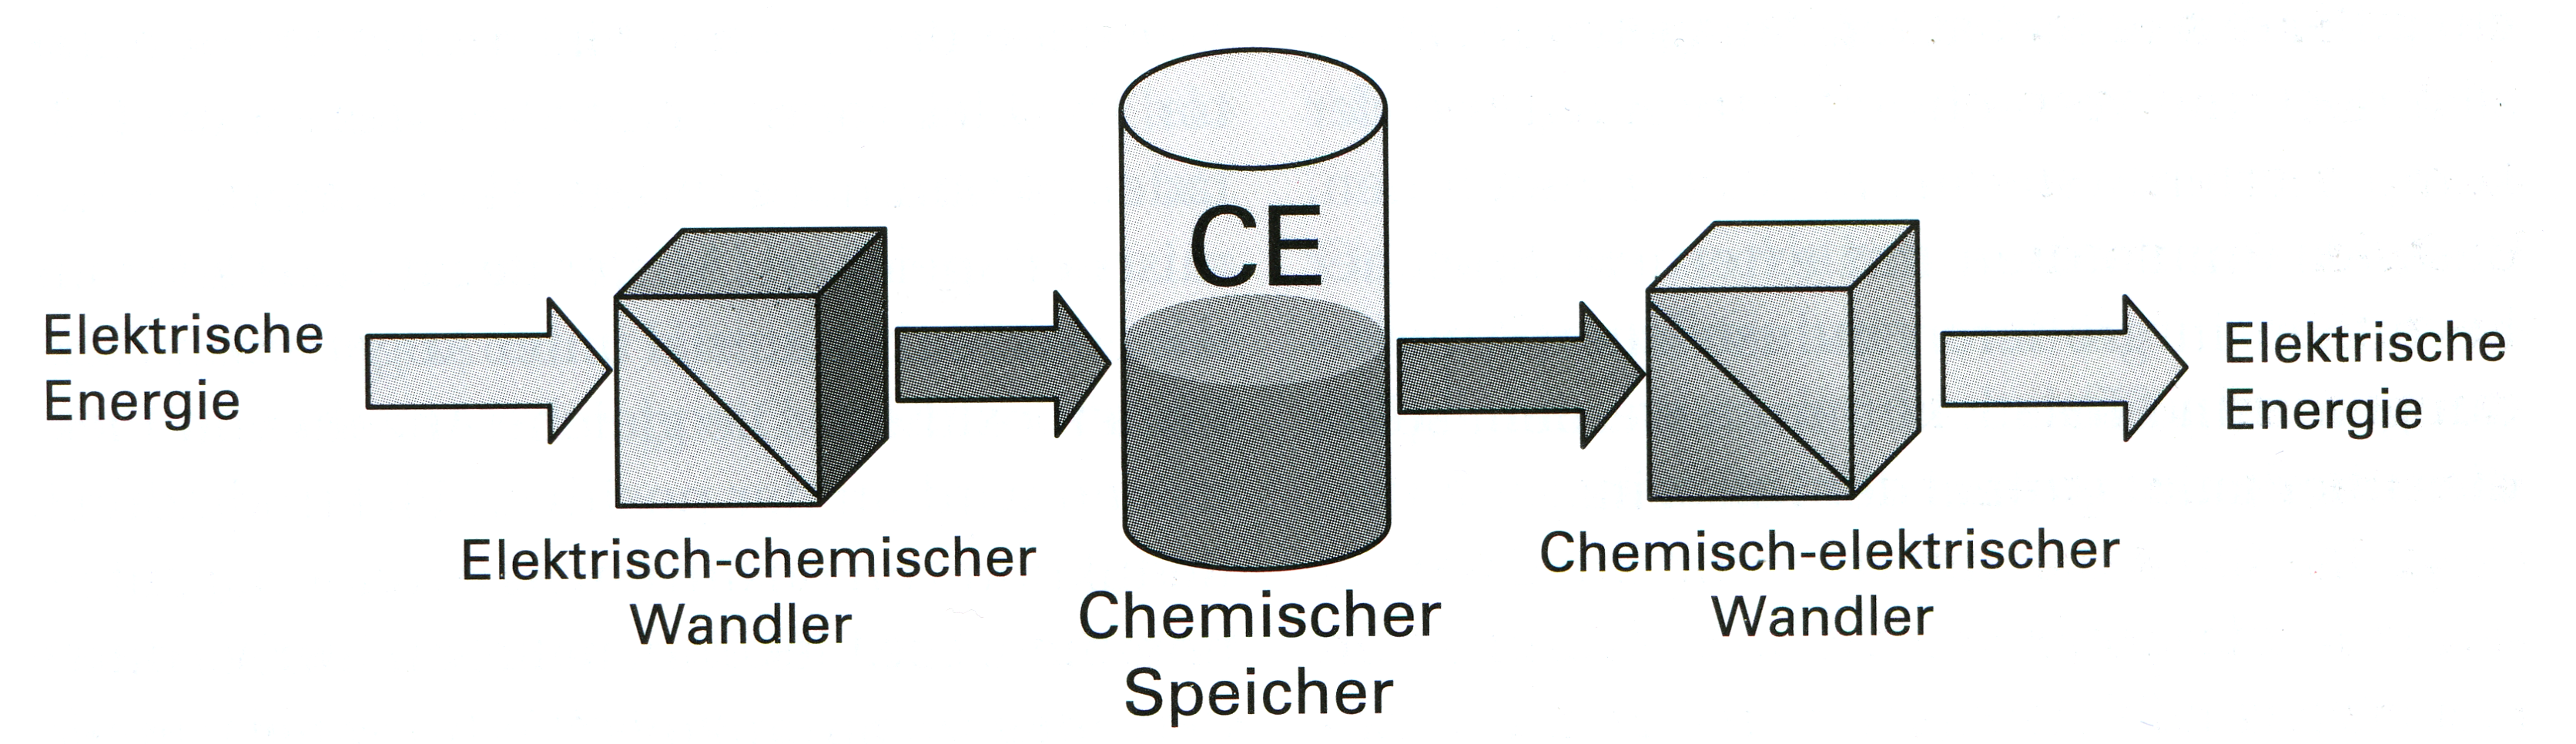
\includegraphics[width=1.0\columnwidth]{images/Prinzipieller_Aufbau.png}
	\caption{Prinzip einer sekundären Zelle}
	\label{Prinzip_Zelle}
\end{figure}
Die Batteriezelle ist eine Form der Galvanischen Zelle. Es lassen sich dabei grundsätzlich drei verschiedene Arten von Galvanischen Zellen unterscheiden:
\begin{description}
\item[Primäre Zelle - Batterie] Primäre Zellen besitzen ein chemisches Potential, welches durch den Anschluss eines externen Verbrauchers als elektrischer Strom abgerufen werden kann. Dieser Vorgang ist jedoch nicht reversibel.
\item[Sekundäre Zelle - Akkumulator] Im Gegensatz zur primären Zelle kann die sekundäre Zelle Energie nicht nur abgeben, sondern auch wieder aufnehmen und speichern. Dieses Verhalten wird in Abbildung \ref{Prinzip_Zelle} dargestellt.
\item[Tertiäre Zelle - Brennstoffzelle] Die Tertiäre Zelle wird kontinuierlich mit einem Brenngas durchflossen und kann daher auch dauerhaft Energie in Form von elektrischen Strom abgeben.  
\end{description}
Die Bezeichnung Akkumulator ist dabei gerade im englischen Sprachgebrauch nicht geläufig, man spricht eher von \textit{rechargeable batteries}, also wiederaufladbaren Batterien. Auch im deutschen geht man dazu über den Begriff Batterie sowohl für primäre als auch für sekundäre Zellen zu gebrauchen. Iim Rahmen dieser Arbeit wird das Wort \textit{Batterie} synonym für beide Arten von Zelle verwendet. Betrachtet werden jedoch nur wiederaufladbare Batterien.
\subsection{Elektrochemischer Vorgang}
\begin{figure}
	\centering
	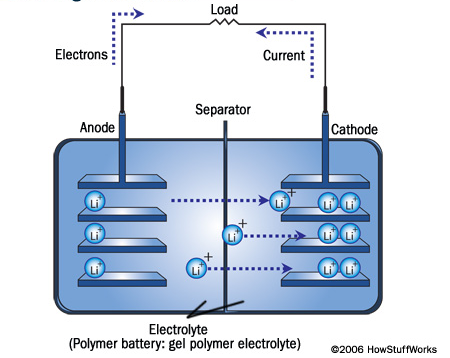
\includegraphics[width=0.6\columnwidth]{images/Schematischer_Aufbau_Li_Ionen.png}
	\caption{Schematischer Aufbau einer Lithium-Ionen-Batterie}
	\label{schema_li_ionen}
\end{figure}
Die Elektrochemie einer Batteriezelle basiert auf einem Potential zwischen zwei räumlich getrennten Materialien. Durch den Anschluss eines externen Stromkreises kann dieses Potential entweder unter Abgabe von Energie abgebaut oder unter Zugabe von Energie vergrößert werden. 
\\\\
Es existieren zwei grundsätzliche Mechanismen zur Ladungsübertragung und Speicherung:
\\\\ %Besser: Unterschiedung reiner Einbau vs. Neubildung von Struktur ???
\textbf{i) Interkalation}
\\\\
Bei der Interkalation handelt es sich um den reinen Einbau eines Atoms oder Ions in ein Wirtsgitter hinein, ohne das Stattfinden einer Reaktion. Beispiel wäre hier der Einbau von Lithiumkationen in eine Graphitstruktur. Bei einer Interkalation kommt es nicht zum Übertrag von Elektronen.
\\\\
\textbf{ii) Redoxreaktion}
\\\\
Während der Redoxreaktion kommt es zu einem Austausch von Elektronen zwischen verschiedenen Edukten. Der reduzierte, also elektronenabgebende, und der oxidierte, also elektronenaufnehmende, Part können dabei räumlich getrennt in den jeweiligen Elektroden vorliegen.
\\\\
Im Falle einer \ce{LiCoO2}-Batterie mit graphitischer Anode wären die bei der Entladung ablaufenden Reaktionen \cite{minakshi2008book}:
\\\\
An der Anode:\\ %Das mit der Interkalation dringend nochmal recherchieren!!!
\begin{equation}
	\ce{Li1C6 -> C6 + Li+ + e-}
\end{equation}
An der Kathode:\\ %Kein vollständiger Ausbau! Korrigieren!
\begin{equation}
	\ce{Li+ + e- + CoO2 -> LiCoO2}
\end{equation}
\subsubsection{Bestimmung der Potentialdifferenz}
Das Potential zwischen zwei Materialien kann als Differenz ihrer jeweiligen Nernstschen Halbzellenpotentiale bestimmt werden. Die Nernst-Gleichung definiert:
\begin{equation}
E = E_0 + \frac{RT}{z_eF}\; ln \frac{a_{Ox}}{a_{Red}}
\end{equation}
mit:
\begin{description}\itemsep0pt
\item[E] Elektrodenpotential
\item[E$_0$] Standardelektrodenpotential
\item[R] Gaskonstante
\item[T] absolute Temperatur
\item[z$_e$] Anzahl der übertragenen Elektronen
\item[F] Faraday-Konstante
\item[a] Aktivität des betreffenden Redox-Partners
\end{description}
Das Verhältnis der Aktivitäten kann dabei als Konzentrationsverhältnis der beiden Phasen dargestellt werden. Einsetzen der Naturkonstanten ergibt als vereinfachte Formel unter der Bedingung eines Betriebes bei Raumtemperatur:
\begin{equation}
E = E_0 + \frac{0,059 V}{z_e} \; log \frac{c_{Ox}}{c_{Red}}
\end{equation}
Über die molare freie Reaktionsenthalpie $\Delta G_m$ kann die Potentialdifferenz als theoretische Zellspannung ebenfalls dargestellt werden:
\begin{equation}
\Delta U_{theo} = -\frac{\Delta G_m}{z_eF}
\end{equation}
Eine einfache Darstellung ist die Angabe des Potentials jedes Stoffes zu reinem Lithiummetall. Die Leerlaufspannung einer Vollzelle ergibt sich dann aus der Differenz zwischen Kathoden- und Anodenspannung gegenüber Lithiummetall:
\begin{equation}
U_{Zelle} = U_{Kathode} - U_{Anode}
\end{equation}
So gilt für eine \ce{LiCoO2}-Zelle mit graphitischer Anode ein mittleres Elektrodenpotential der Kathode gegen Lithium von 3,9V, der Anode von ungefähr 0,1V. Die Zelle erreicht daher eine theoretische Zellspannung von 3,8V.
\subsection{Aufbau}
Eine Batterie besteht aus zwei räumlich voneinander getrennten Elektroden. Dabei wird die Elektrode mit dem niedrigeren Halbzellenpotential als Anode, die Elektrode mit dem höheren Halbzellenpotential als Kathode bezeichnet. Zwischen den beiden Elektroden existiert ein Elektrolyt. Dieser ermöglicht den Ladungsaustausch beider Elektroden über den Transfer von Ionen. Um einen Kurzschluss, also einen direkten Ladungsaustausch zwischen beiden Elektroden, zu vermeiden, kann es außerdem nötig sein, einen Separator zwischen beiden Elektroden einzusetzen. Die beiden Elektroden sind jeweils auf einem Stromkollektor aufgebracht, welcher die Kontaktierung der Elektrode nach außen hin ermöglicht.
\\\\
Es gibt verschiedene Bauformen für Batteriezellen.
\begin{figure}
	\centering
	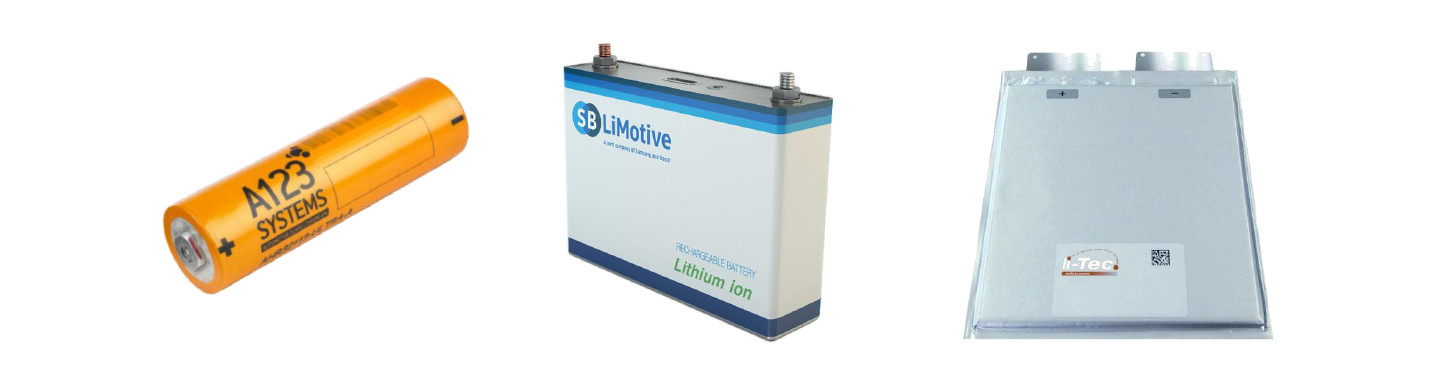
\includegraphics[width=1.0\columnwidth]{images/rund_prisma_pouch.jpg}
	\caption{Vergleich möglicher Bauformen: Rundzelle, prismatische Zelle, Pouch-Zelle}
	\label{vergleich_zellform}
\end{figure}
\begin{description}
\item[Rundzellen] Bei der Rundzellen werden die Stromkollektoren jeweils doppelseitig mit einem Elektrodenmaterial beschichtet und dann abwechselnd aufeinander gestapelt. Anschließend wird die Batteriezelle zu einem Zylinder aufgewickelt.
\item[Prismatische Zellen] Die prismatische Zelle ähnelt im Aufbau der Rundzelle, wird jedoch rechteckig gewickelt und ist so besser schichtbar.
\item[Pouch-Zellen] In diesen Zellen werden meist nur wenige Schichten von Elektroden übereinander gewickelt und anschließend in einer dünnen Hülle gasdicht verschweißt. Ein vor dem Einschweißen durchgeführtes Anbringen eines Vakuums garantiert das Entfernen überflüssiger Gase innerhalb der Zelle.
\item[Knopfzellen] In einer Knopfzelle werden die Elektroden, Elektrolyt und Separator jeweils rund geformt auf einem Boden gestapelt und anschließend mit einem Deckel verschlossen. Eine zusätzlich eingebrachte Feder zwischen Zelle und Deckel sorgt für den notwendigen Anpressdruck, um eine gute Kontaktierung zu gewährleisten.
\end{description}
Eine Übersicht über die verschiedenen Bauformen wird in Abbildung \ref{vergleich_zellform} gezeigt. Batteriezellen können zu Batteriemodulen zusammengeschlossen werden, die dann über ein externes Batteriemanagement gezielt angesprochen und kontrolliert werden können. Ein solcher Aufbau ist in Abbildung \ref{battery_pack} zu sehen.
\\\\
Am IAM-KWT kommen spezielle Testzellen zum Einsatz, deren Aufbau dem von Knopfzellen ähnelt. Die beiden Elektroden und der Elektrolyt werden in eine Glasröhre übereinander montiert. Die Röhre ist über zwei Stopfen mit Dichtungsringen nach außen hin abgedichtet. Eine Druckfeder sorgt für den nötigen Anpressdruck, zwei Edelstahlplättchen für eine homogene Kraftverteilung und Kontaktierung. Verschlossen wird die Zelle mittels Plastikverschlüssen, welche die Stopfen am Verrutschen hindern. Über einfache 2mm-Bohrungen in den Stopfen kann die Zelle mit Bananensteckern an Geräte angeschlossen werden. Die Abbildung \ref{schema_zelle} zeigt die Testzelle schematisch.
\begin{figure}
	\centering
	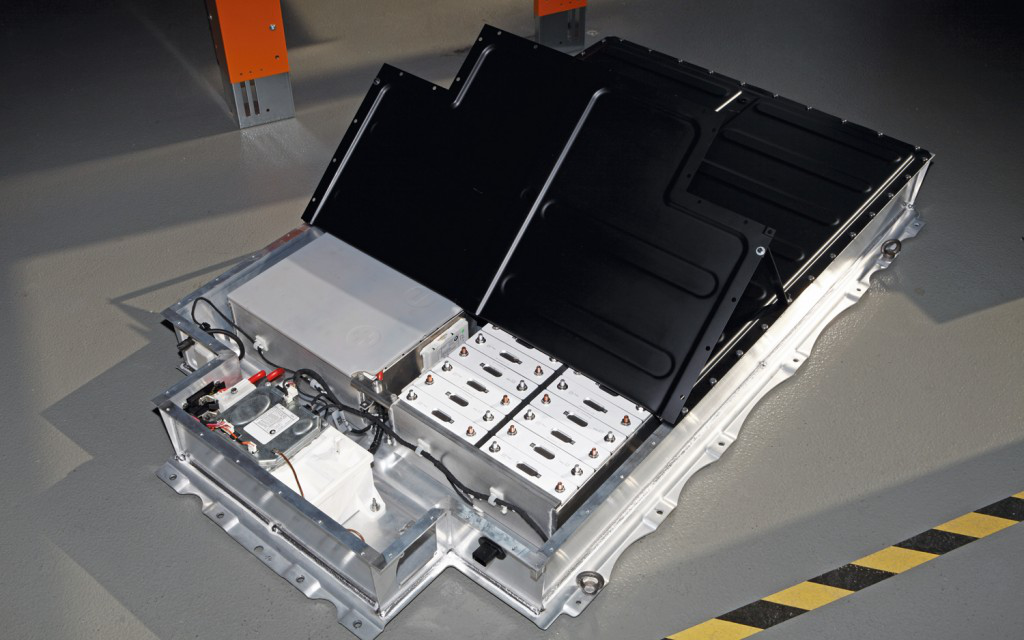
\includegraphics[width=0.9\columnwidth]{images/bmw-i3-battery-pack.png}
	\caption{Battery-Pack des BMW i3 bestehend aus zwei Batteriemodulen und einem Batteriemanagement}
	\label{battery_pack}
\end{figure}
\begin{figure}
	\centering
	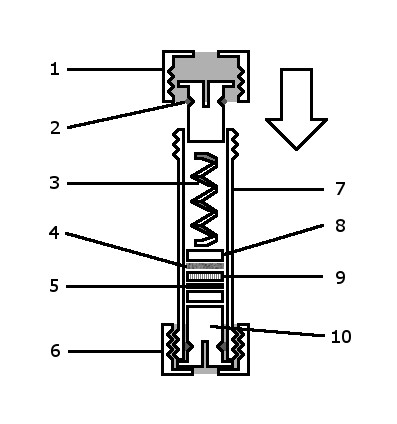
\includegraphics[width=0.55\columnwidth]{images/Schema_Zelle.jpg}
	\caption{Schema der IAM-KWT-Testzelle; 
			1: Plastikkappe,
			2: Dichtungsring,
			3: Edelstahlfeder,
			4: Kathode,
			5: Anode,
			6: Plastikkappe,
			7: Glaszylinder,
			8: Kontaktierplättchen,
			9: Separator,
			10: Edelstahlstopfen.
			}
	\label{schema_zelle}
\end{figure}
\subsection{Elektrodenmaterialien}
Materialien müssen verschiedene chemische und physikalische Eigenschaften erfüllen, um für den Einsatz in Elektroden geeignet zu sein. Die eingesetzten Stoffe sollten ungiftig sein und in ausreichender Menge günstig zu beschaffen sein. Sie sollten eine ausreichend hohe Potentialdifferenz zwischen den Elektroden besitzen, um eine hohe Zellspannung gewährleisten zu können. Das Material sollte eine möglichs hohe Energie- und Leistungssdichte ermöglichen, um auch für den mobilen Einsatz interessant zu sein. Es muss sowohl eine gute Lithium- als auch Elektronenleitfähigkeit gewährleistet sein. Die Ein- und Auslagerung von Lithium sollte nicht zu einer zu hohen Veränderung des Volumens führen, da diese unter Umstände Grenzflächen zerstört und hohe Anforderungen an die Bauweise der Zellen stellt. Auch nach einer hohen Anzahl an Zyklierungen sollte das Material noch eine ausreichende Kapazität besitzen. Ein Versagen der Zelle sollte möglichst nicht zu einer starken Hitzeentwicklung und Explosion der Zelle führen.
\\\\
Die Materialien für Elektroden können grundsätzlich nach ihrem Diffusionsverhalten klassifiziert werden.
\begin{description}
\item[Olivinstruktur] Die Olivinstruktur ist eine eindimensionale Tunnelstruktur, an der entlang die Diffusion stattfindet.
\item[Lagenstruktur] Materialien, die zweidimensionale Diffusion zwischen Schichten ermöglichen, besitzen eine Lagenstruktur.
\item[Spinellstruktur] In der Spinellstruktur ist eine Diffusion in alle drei Richtungen des Raums möglich.
\end{description}

\begin{figure}
	\centering
	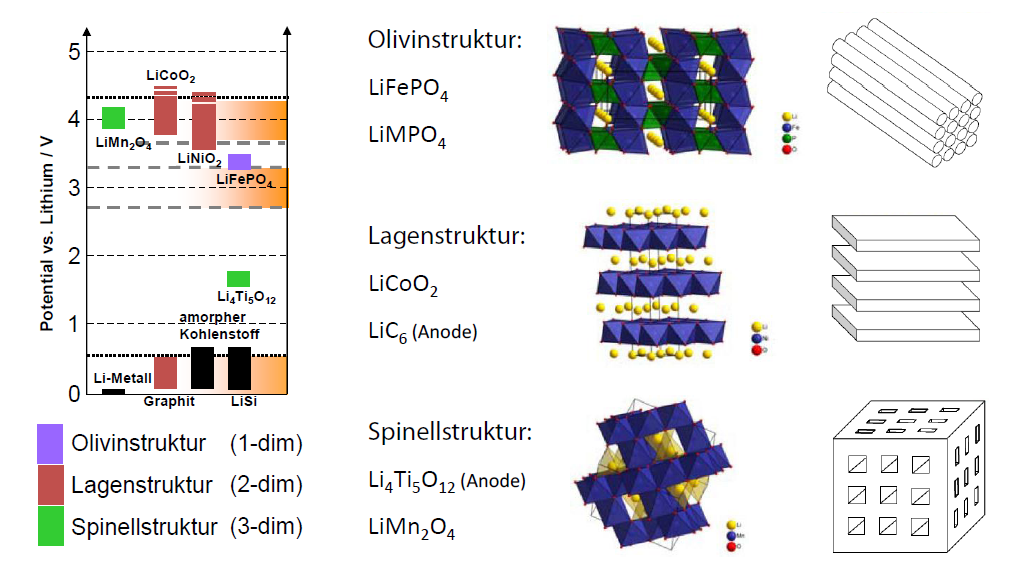
\includegraphics[width=1.0\columnwidth]{images/strukturen_elektroden.png}
	\caption{Spannunglsagen verschiedener Elektrodenmaterialien (links) und ihre entsprechenden Kanalstrukturen (rechts) (BuB-Skript)}
	\label{strukturen_elektroden}
\end{figure}
\subsubsection{Typische Anodenmaterialien}
% Was zur SEI schreiben? Quelle Skript BuB?
Für die meisten Zellen in dieser Arbeit kamen metallische Lithiumanoden zum Einsatz. Kommerziell ist Graphit momentan das Standardanodenmaterial von Lithium-Ionen-Batterien.
\begin{description}
\item[Lithium-Metall] Rein metallisches Lithium besitzt eine sehr hohe theoretische Kapazität von 3860mAh/g. Da jedoch die Anode im Betrieb nicht aufgebraucht werden darf, muss es im Überschuss bereit gestellt werden. Es besitzt die maximal mögliche Zellspannung gegenüber der Kathode. Problematisch ist jedoch, dass es durch das fehlende Wirtsgitter dazu neigt während der Zyklierung Dendriten auszubilden, die schlussendlich zu einem Kurzschluss und Ausfall der Zelle führen.
\item[Graphit (\ce{C6})] Graphit besitzt eine Lagenstruktur zwischen der er Lithium einspeichern kann. Es kann jeweils ein Lithiumatom pro sechs Kohlenstoffatomen eingelagert werden. Er erreicht damit eine theoretische Kapazität von 372 mAh/g. Das Potential gegen rein metallisches Lithium ist sehr klein (ca. 0,1V), was hohe Zellspannungen ermöglicht. Die Einlagerung erfolgt über drei unterschiedliche Stufen und führt zu einer Volumenzunahme von maximal 9\%.
\item[Lithiumtitanat (\ce{Li4Ti5O12}, LTO)] Teilweise auch Lithiumtitanspinell. Lithiumtitanat besitzt eine Spinellstruktur. Die theoretische Kapazität liegt bei 233mAh/g, in der Praxis werden meistens Kapazitäten von etwa 150mAh/g erreicht. Das Material vollführt nahezu keine Volumenänderung bei Ein- und Ausbau von Lithium. Jedoch ist seine Potentiallage mit 1,55V gegenüber metallischem Lithium sehr hoch, was zu kleineren Zellspannungen führt.
\end{description}
\subsubsection{Typische Kathodenmaterialien}
\begin{description}
\item[Lithiumcobaltdioxid (\ce{LiCoO2})] Die praktische Kapazität von Lithiumcobaltoxid liegt bei 150mAh/g. Dies liegt an der Tatsache, dass nur etwa 60\% der Lithiumatome aus dem Gitter ausgebaut werden dürfen, da es sonst durch den Zusammenbruch der Struktur zur Bildung von Sauerstoff kommt. Beim Laden muss daher die Spannung unter 4,2V gehalten werden. Die Diffusion läuft daher zweidimensional zwischen zwei Schichten ab. Das mittlere Elektrodenpotential von Lithiumcobaltoxid liegt bei hohen 3,9V.
\item[Lithiummanganspinell (\ce{LiMn2O4}, LMO)] Lithiummanganspinell ist ein Hochvolkathodenmaterial, sein mittleres Elektrodenpotential liegt bei 4,0V. Die praktische Kapazität des Stoffes liegt bei etwa 120mAh/g bei der Verwendung von Flüssigelektrolyten, welche die Ladespannung auf 4,2V begrenzen. Der Spinell selbst ist auch noch bei höheren Potentialen stabil. Bei tiefen Ladezuständen kann es zu einer Manganauslösung und unerwünschten Gitterumwandlungen kommen, der Jahn-Teller-Verzerrung. Um diese zu verhindern, können Teile des Mangans durch andere Übergangsmetalle substituiert werden. In dieser Arbeit wird eine \ce{LiNi_{0,5}Mn_{1,5}O4}-Verbindung (LNMO) untersucht.
\item[Schwefel] Reiner Schwefel besitzt normalerweise einen zyklischen Achterring. Beim Einsatz als Kathodenmaterial wird dieser Ring beim Entladen langsam reduziert und es entstehen verschiedene Polysulfide:
\begin{equation}
\begin{split}
\ce{S8 -> Li2S8 -> Li2S6 -> Li2S6 -> Li2S5 -> }\\
\ce{ Li2S4 -> Li2S3 -> Li2S2 -> Li2S}
\end{split}
\end{equation}
Diese existieren in unterschiedlichen Konzentrationen auch nebeneinander, der Schwefelanteil am Gemisch nimmt aber während dem Entladevorgang ab. Dieser Vorgang findet reversibel beim Laden der Zelle statt. Die theoretische Kapazität einer Lithium-Schwefel-Zelle liegt bei 1672mAh/g, praktisch kann aber momentan bei höheren Lade/Entladeraten jedoch nur ein um den Faktor 5-10 niedrigerer Wert erreicht werden. Das größte Problem des Materials sind ungewollte Reaktionen der Polysulfide mit dem Elektrolyten und eine damit einhergehende schleichende Vergiftung des Elektrolyten und Verlust an Aktivmaterial.
\end{description}
Alle Kathodenmaterialien und auch das Anodenmaterial LTO besitzen eine zu schwache Leitfähigkeit für Elektronen. Daher wird ihnen Kohlenstoff beigemischt, um Elektronen in die Elektrode zu transportieren. Die Materialien werden dabei mit Bindern versetzt. Die optimale Auswahl an Kohlenstoffmodifikation (Ruß, Graphit, Kohlenstoffnanoröhrchen, Graphen) und deren Prozessierung ist dabei eine aktuelle Forschungsaktivität (QUELLE). Es wird eine möglichst geringe Beimischung dieser Zusatzstoffe angestrebt, um die Masse an Aktivmaterial in der Zelle zu optimieren.
\subsection{Elektrolyte}
\begin{figure}
	\centering
	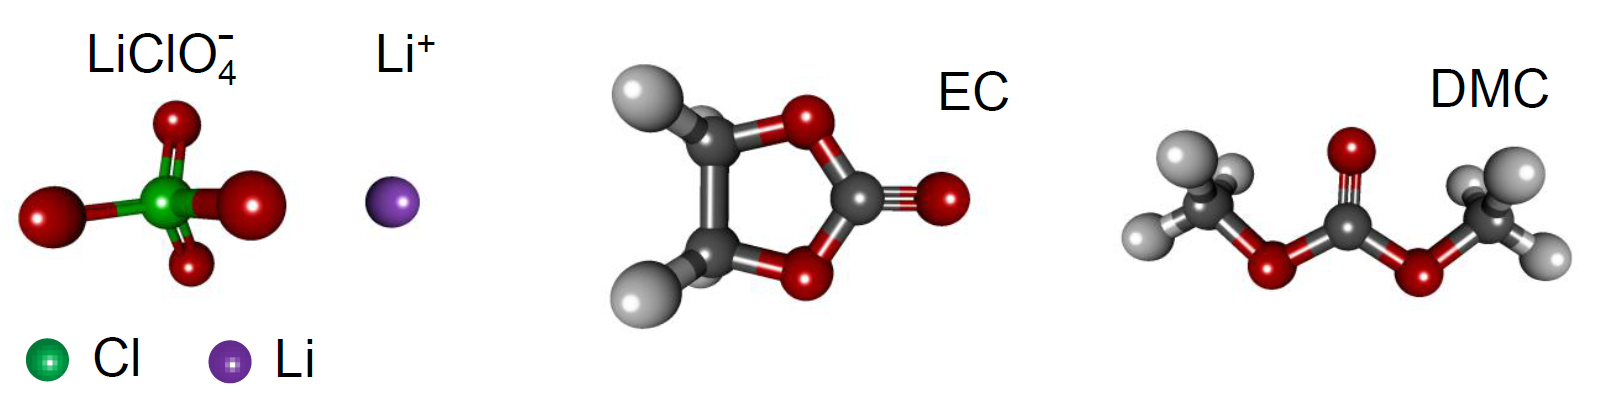
\includegraphics[width=1.0\columnwidth]{images/fluessigelektrolyt.png}
	\caption{Chemische Strukturen der Bestandteile eines Flüssigelektrolyten}
	\label{fluessigelektrolyt}
\end{figure}
Elektrolyte sollen möglichst wenig elektronenleitend sein, um eine schleichende Selbstentladung der Batterie zu verhindern. Gleichzeitig muss aber eine gute Ionenleitfähigkeit gewährleistet werden, um eine hohe Leistung der Zelle zu ermöglichen. Weiterhin müssen die Grenzflächen zwischen Elektrode und Elektrolyt eine ausreichende Güte besitzen, damit die Ionen zwischen beiden Zellbestandteilen wandern können.
\\\\
Als Elektrolyt kommen kommerziell fast ausschließlich Flüssigelektrolyte zum Einsatz. Diese bestehen aus einem organischen Lösungsmittel wie beispielsweise einer Ethylencarbonat-Dimethylcarbonat-Mischung (EC-DMC). Hier sorgt das stark polare Ethylencarbonat für die Löslichkeit, während man mit dem Dimethylcarbonat-Anteil die Viskosität der Lösung einstellen kann. In diese Mischung löst man dann ungesättigte Lithium-Leitsalze wie \ce{LiPF6}, \ce{LiAsF6} oder \ce{LiClO4}. Eine Abbildung der chemischen Strukturen der Bestandteile eines Flüssigelektrolyten auf EC/DMC-Basis mit \ce{LiClO4} als Leitsalz ist in Abbildung \ref{fluessigelektrolyt} dargestellt.
\\\\
Problem dieser Lösungen sind ihre schlechte Beständigkeit gegenüber Wasser. Bei \ce{LiPF6} sorgen beispielsweise schon kleinste Verunreinigungen des Elektrolyts zur Bildung von hochätzender Flusssäure, die den Elektrolyt vergiftet und zu einem Ausfall der Zelle führt. Dies ist bei der Herstellung von Lithium-Ionen-Batterien ein großes Problem, da es eine aufwendige und teure Trocknung der Luft bei der Herstellung der Zellen erfordert.
\\\\
Ein weiteres Problem von Flüssigelektrolyten ist ihr begrenztes Temperaturfenster. Bei zu hohen Temperaturen verdampft der Elektrolyt und zerstört so die Zelle, bei zu niedrigeren Temperaturen bildet sich zumeist ein Polymergel, welches nicht mehr in der Lage ist die Ionen zu leiten.
\section{Keramiken}
Keramiken sind anorganische, nicht-metallische und polykristalline Werkstoffe. Es existieren verschiedene Keramiken, welche in der Lage sind Lithium-Ionen zu leiten. Grundsätzlich lassen sich dabei basierend auf der Struktur der Werkstoffe zwei vielversprechende Klassen von lithiumleitenden Keramiken identifizieren: Die perowskitischen sowie die Na-Super-Ionic-Conductor (NASICON) Keramiken. 
\subsection{Perowskite}
\begin{figure}
	\centering
	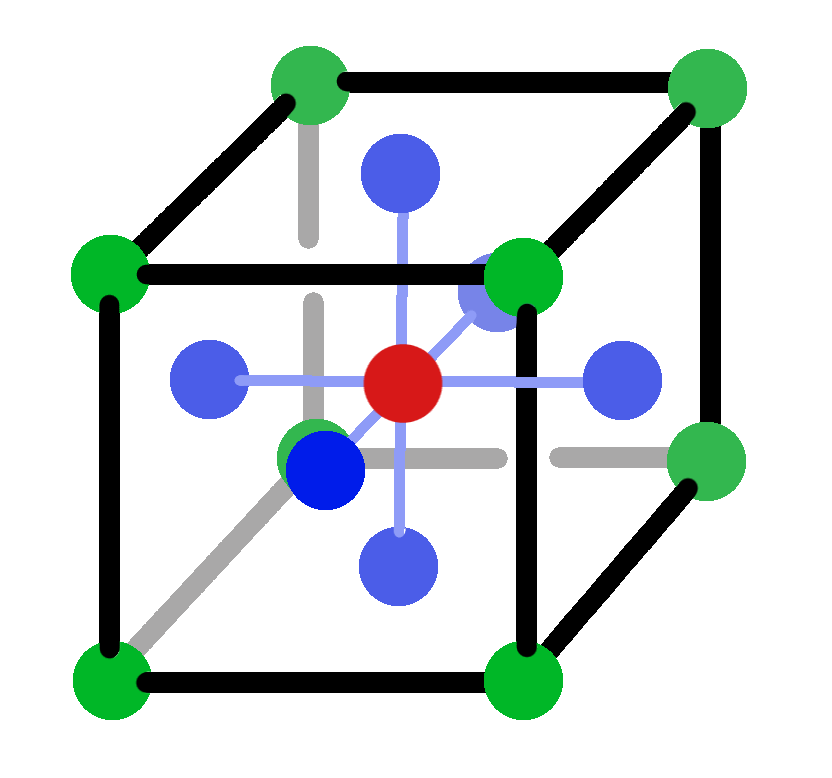
\includegraphics[width=0.5\columnwidth]{images/Perowskit-Struktur.png}
	\caption{\ce{ABO3}-Struktur eines Perowskits (blau: A, rot: B, grün: O)}
	\label{struktur-perowskit}
\end{figure}
Perowskite folgen der Struktur \ce{ABO_3}. Sie sind kubisch-flächenzentriert aufgebaut mit dem B-Element in der Mitte, den A-Elementen an den Ecken und dem Sauerstoff auf den Flächen. Der Sauerstoff ist zweifach negativ geladen. Damit ergibt sich für die Kombination aus A und B eine notwendige sechsfach positive Gesamtladung.
\\\\
Ein vielversprechendes Material für den Einsatz als Festkörperelektrolyt ist hier das Lithiumlanthantitanoxid (\ce{LiLaTiO3}, LLTO). Das einfach positive Lithium und das dreifach positive Lanthan besetzen dabei die A-Plätze, das vierfach positive Titan den B-Platz. Mögliche Strukturen des LLTO können daher über die Formel \ce{Li_{3x}La_{2/3-x}TiO3} mit $x \in (0, 1/6)$ beschrieben werden. Der Anteil an Leerstellen in der Struktur steigt mit größerem x an.
\\\\
Durch die Leerstellen auf den A-Plätzen und durch Diffusion können Lithiumionen durch das Material wandern. Dabei bilden jeweils vier Sauerstoffionen eine Flaschenhalsformation (QUELLE). Durch eine unterschiedliche Neigung der TiO6-Oktaeder ist der Diffusionswiderstand und die Aktivierungsenergie allerdings im Material inhomogen verteilt. Da sich im Material außerdem entlang der c-Achse lanthanreiche und lanthanarme Schichten bilden, ist die Leerstellenbewegung zwischen diesen Ebenen teilweise gehemmt (QUELLE).
\\\\
Für Lithiumlanthantitanoxid konnte eine Bulk-Leitfähigkeit von bis zu 1x$10^{-3}$ S/cm nachgewiesen werden (QUELLE), weshalb eine Einsatzmöglichkeit als Festkörperelektrolyt untersucht wird.
\subsection{NASICON-Keramiken}
Das Akronym NASICON steht für \textbf{Na}-\textbf{S}uper-\textbf{I}onic-\textbf{Con}ductor und wurde ursprünglich für spezielle, natriumleitende Keramiken in Natrium-Schwefel-Batterien verwendet. Heute steht es allerdings für eine ganze Klasse an Keramiken die mit der allgemeinen Formel \ce{LiM2(PO4)3} beschrieben werden können. Dabei steht der Platzhalter M für ein Element aus der Gruppe Titan (Ti), Zirkon (Zr), Germanium (Ge) oder Hafnium (Hf).
\\\\
Die Struktur der NASICON-Keramiken ist aus \ce{MO6}-Oktaedern und \ce{PO4}-Tetraedern aufgebaut. Dabei verbindet sich ein \ce{PO4}-Tetraeder immer mit vier unterschiedlichen \ce{MO6}-Oktaedern, der wiederum mit sechs unterschiedlichen Tetraedern in Kontakt steht. Zwischen dieser Struktur existieren zwei Zwischengitterplätze, auf dem sich die Lithiumionen aufhalten können. Eine Darstellung ist in Abbildung (noch einfügen) ersichtlich.
\\\\
Der Zwischengitterplatz M1 beschreibt dabei einen Raum zwischen zwei \ce{MO6}-Oktaedern entlang der c-Achse. Die M2-Plätze sind hingegen senkrecht zur c-Achse zwischen den Bändern angeordnet. Zwischen diesen Räumen existieren außerdem noch M12 Plätze. Von entscheidender Bedeutung für die Leitfähigkeit des Materials ist nun, welche Größe die Engstelle zwischen den Gitterplätzen einnimmt. Dieser Flaschenhals kann maßgeblich durch die Ionen innerhalb der Gitterstruktur beeinflusst werden.
\subsubsection{Lithiumtitanphosphat}
Wählt man als Komponente M Titan, so erhält man Lithiumtitanphosphat (\ce{LiTi2(PO4)3}). Die zueinander passenden Größen von Lithiumionen auf der einen und der Zwischengitterstruktur auf der anderen Seite sorgt für eine sehr gute Leitfähigkeit. Die Lithiumionen besetzen dabei vollständig die M1-Stellen, die M2-Stellen bleiben vollständig unbesetzt. 
\\\\
Eine weitere Erhöhung der Bulk-Leitfähigkeit kann durch einen teilweisen Einbau von beweglicheren Aluminiumionen anstelle von Titanionen erzielt werden. Das entstehende Material ist Lithium-Aluminium-Titanphosphat (LATP) und kann durch die allgemeine Struktur \ce{Li_{1+x}Al_{x}Ti_{2-x}(PO4)3} beschrieben werden. Die durch die Substituierung der Titanionen zusätzlich eingebrachten Lithiumionen besetzten dabei M2-Plätze, was zu einer Steigerung der Ionenleitfähigkeit führt.
\\\\
Die \ce{Ti^{4+}}-Ionen des LATP werden von verschiedenen Anodenmaterialien, wie Lithiummetall oder lithiierten Graphit, zu \ce{Ti^{3+}} reduziert. Diese Instabilität kann zu einem Versagen des Elektrolyts führen. Das LATP muss daher mit einem geeigneten Anodenmaterial kombiniert werden.
\subsubsection{Lithium-Aluminium-Germaniumphosphat}
Um der Reduktion der Titankationen vorzubeugen, können diese mit Germaniumkationen ersetzt werden. Das so entstehende Material ist Lithium-Aluminium-Germaniumphosphat (LAGP). Es kann mit der allgemeinen Struktur \ce{Li_{1+x}Al_xGe_{2-x}(PO4)3} beschrieben werden.
\\\\
LAGP besitzt eine mit LATP vergleichbare Leitfähigkeit und ist außerdem auch noch bei hohen Spannungen von bis zu 7V stabil gegen Lithium.
% Details zur Herstellung?
\section{Analysemethoden}
Zur Strukturaufklärung werden die Materialien mit drei unterschiedlichen Analysemethoden untersucht. Die Röntgendiffraktion misst Reflexionen und Interferenzen an Kristallgittern und ermöglicht daher eine Charakterisierung der untersuchten Stoffe über ihre kristalline Struktur. Bei der Impedanzspektroskopie wird der frequenzabhängige, komplexe Widerstand eines Materials untersucht, um dessen Leitfähigkeit genauer analysieren zu können. Die Kernspinspektroskopie ermöglicht die genaue Untersuchung der atomaren Umgebung eines speziellen Elements innerhalb einer Struktur durch gezieltes Ausrichten und Variieren der Kernspins.
\subsection{Röntgendiffraktion}
Die Röntgendiffraktion (X-Ray Diffraction, XRD) nutzt den Zustand der charakteristischen Beugung von Röntgenstrahlung an geordneten Strukturen wie Kristallen aus, um daraus Aussagen über diese Struktur treffen zu können. Damit ist es beispielsweise möglich, die Phasenreinheit eines Stoffes zu bestimmen.
\subsubsection{Physikalische Grundlagen der XRD}
Bei der Beugung von Röntgenstrahlen an Kristallgittern entstehen Interferenzen durch die unterschiedlich tiefe Eindringung in das Material bis zum Auftreffen auf ein Teilchen. Dieser Umstand kann mit der Bragg-Gleichung beschrieben werden:
\begin{equation}
n\lambda = 2d \sin{\theta}
\end{equation}
mit
\begin{description}\itemsep0pt
\item[n] Grad des untersuchten Maximums (?)
\item[$\lambda$] Wellenlänge der Röntgenstrahlung
\item[d] Abstand der Netzebenen
\item[$\theta$] Winkel der Strahlung zur Netzebene
\end{description}
Eine schematische Darstellung ist in Abbildung \ref{bragg} gegeben.
% Weitere Beschreibung?
\begin{figure}
	\centering
	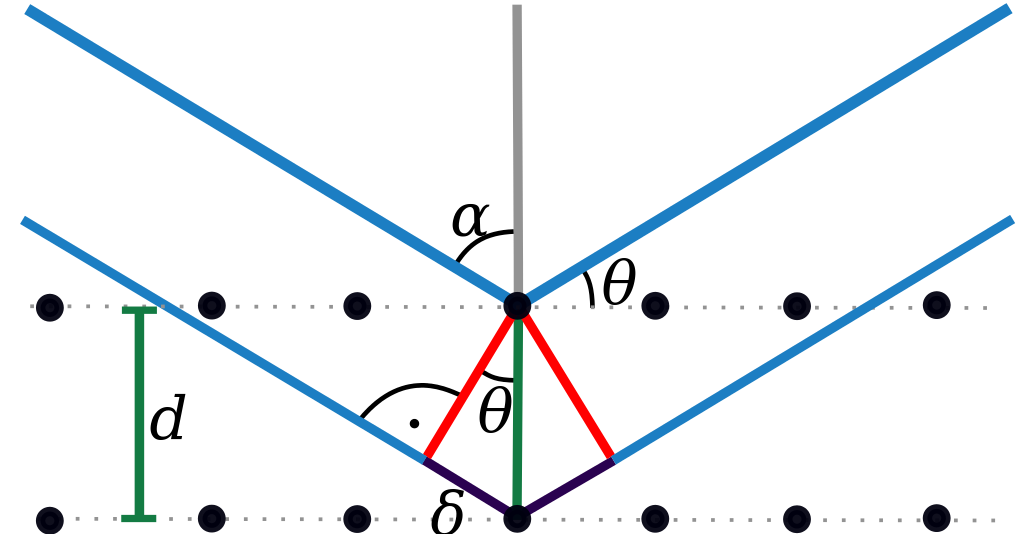
\includegraphics[width=0.6\columnwidth]{images/Bragg.png}
	\caption{Schematische Darstellung der Bragg-Reflexion (https://de.wikipedia.org/wiki/Datei:Bragg.svg)}
	\label{bragg}
\end{figure}
\subsubsection{Bragg-Brentano-Diffraktometer}
Eine Bragg-Brentano-Anordunung eignet sich besonders für das Anfertigen von Pulverdiffraktogrammen. Eine ebene, flache Probe, z.B. in einen kleinen Tigel gepresstes Pulver, wird im Mittelpunkt eines Drehkreises befestigt. Der Röhrenfokus wird nun im gleichen Abstand zur Probe wie der Detektor angebracht. Beide zeigen im gleichen Winkel auf die Probe. Während der Messung wird dieser Winkel nun kontinuierlich variiert. Dazu kann entweder die Probe mit halber Winkelgeschwindigkeit des Detektors gedreht werden oder Röhre und Detektor bewegen sich mit gleicher Geschwindigkeit aufeinander zu beziehungsweise voneinander weg. Es kann nun für jeden Winkel quantitativ das Maß an Reflexion und Interferenz gemessen werden und daraus ein Diffraktogramm erstellt werden. Mittels Rietveld-Methode oder Vergleich mit einer Datenbank ist anschließend eine Analyse des Diffraktogramms möglich.
% Evtl. noch eine Grafik?
\\\\
Die Röntgenbeugungsexperimente wurden am Röntgendiffraktometer D500 der Firma Siemens durchgeführt. %Ggf. in die Methodik stecken
\subsection{Zyklische Voltametrie}
Bei der zyklischen Voltametrie wird zuerst ein ansteigendes und anschließend ein abfallendes Potential an eine Batterie angelegt. Gemessen wird die sich bei den unterschiedlichen Potentialen ergebende Stromstärke. Diese ist ein Maß dafür, ob eine elektrochemische Reaktion innerhalb der Batterie stattfindet. Diese stellt sich als ein Peak innerhalb des Diagramms der zyklischen Voltametrie dar. Es kann dabei zwischen oxidierenden und reduzierenden Reaktionen unterschieden werden, je nachdem ob ein Peak im ansteigenden oder im abfallenden Potentialbereich auftritt.
\\\\
Die zyklische Voltametrie ist insbesondere dazu geeignet, zu verstehen bei welchen Spannungen Reaktionen ablaufen und ermöglicht damit das exakte einstellen von Arbeitsspannungen zum Laden und Entladen von Batteriezellen, die nicht über- oder unterschritten werden sollten.
\subsection{Impedanzspektroskopie}
Die Impedanzspektroskopie eignet sich, um Widerstände in einem Gesamtsystem genauer zu untersuchen und dadurch Aussagen über die Leitung innerhalb des Systems treffen zu können.
\subsubsection{Grundlagen der Impedanzspektroskopie}
Kapazitive und induktive Bauelemente besitzen einen sich über den Zeitverlauf ändernden Widerstand. Werden diese nun in einem Wechselstrom betrieben, so entsteht ein frequenzabhängiger Widerstand, die Impedanz. Eine Impedanz ist aufgebaut aus einem realen, frequenz\-unabhängigen und einem komplexen, frequenz\-abhängigen Teil.
\\\\
Admittanz, Leitfähigkeit.
\subsubsection{Elektrochemisches Ersatzschaltbild}
\begin{figure}
	\centering
	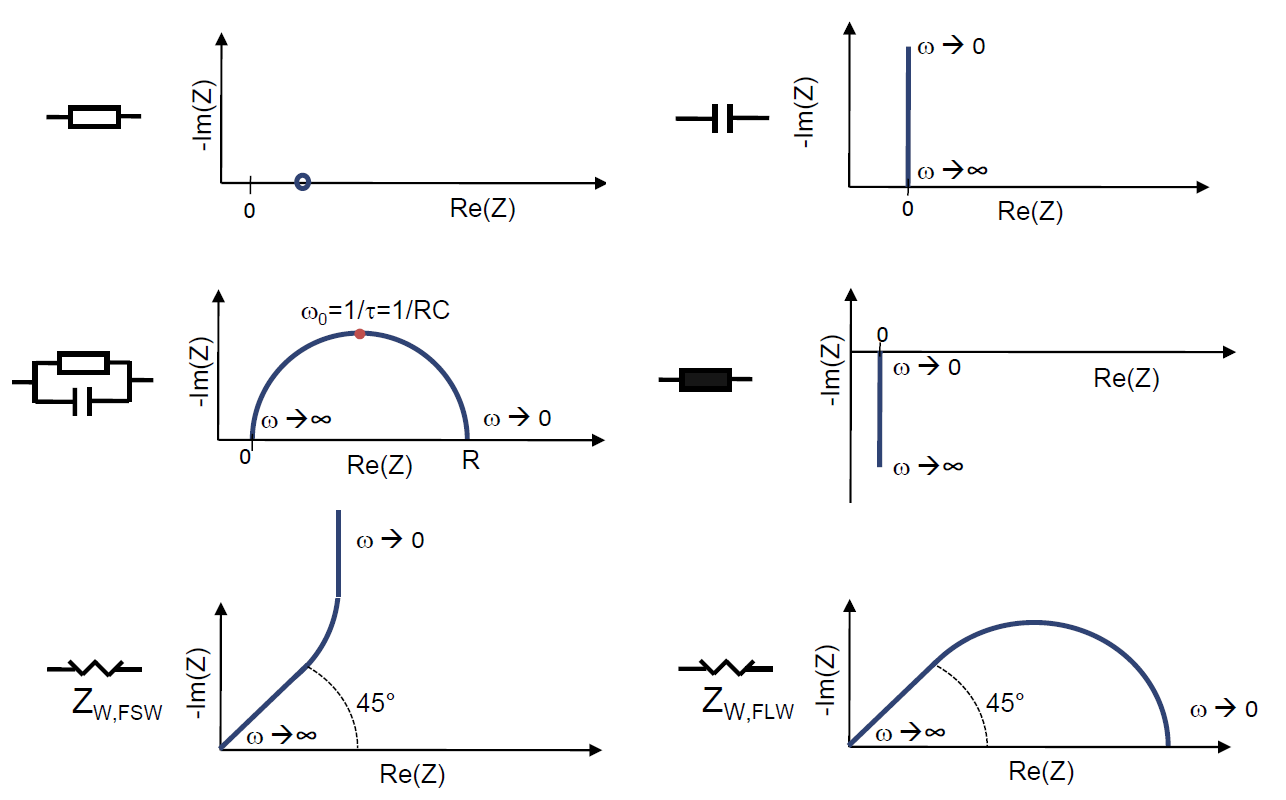
\includegraphics[width=1.0\columnwidth]{images/is_bauteile.png}
	\caption{Ideale Darstellung verschiedener elektrotechnischer Bauteile bei der Impedanzspektroskopie im Nyquist-Plot}
	\label{bauteile_is}
\end{figure}
Elektrotechnische Bauelemente besitzen nun unterschiedliche, charakteristische Impedanzen. Eine Verschaltung unterschiedlicher Elemente resultiert in einem Impedanzspektrum. Dargestellt werden können diese in einem Nyquist-Plot, der den Realteil gegen den Imaginärteil aufträgt. Eine Übersicht über alle Bauteile und ihre korrespondierenden Nyquist-Plots findet sich in Abbildung \ref{bauteile_is}.
\begin{description}
\item[Widerstand] Der Widerstand besitzt keinen komplexen, sondern lediglich einen realen Anteil. Dies entspricht einem Punkt auf der Realachse des Nyquist-Plots.
\item[Kondensator] Ein idealer Kondensator besitzt keinen realen Widerstand. Sein Imaginärteil konvergiert bei hohen Frequenzen gegen Null, bei niedrigen Frequenzen divergiert er ins Negative.
\item[Spule] Eine Spule besitzt ebenfalls keinen realen, sondern nur einen imaginären Widerstand. Dieser konvergiert für niedrige Frequenzen gegen Null, bei hohen Frequenzen divergiert er ins Positive
\item[RC-Glied] Grenzflächen, beispielsweise zwischen Elektrode und Elektrolyt in einer Batterie, bilden meistens sogenannte Helmholtz-Doppelschichten aus. Sie besitzen sowohl ein kapazitives Element als auch einen Durchtrittswiderstand. Dies kann als RC-Glied, also einer Parallelschaltung von Widerstand und Kondensator, dargestellt werden. Im Nyquist-Plot ergibt sich ein Halbkreis mit Radius 1/RC.
\item[Warburg-Element] Um Diffusionprozesse darzustellen, können Warburg-Elemente verwendet werden. Diese leiten sich aus den Fickschen Gesetzen her. Sie bestehen aus einem Kettenleitermodell aus Widerständen und Kondensatoren, wobei zwischen Finite-Length und Finite-Space Warburg-Elementen unterschieden werden muss (siehe Abbildung \ref{warburg_element})
\end{description}
\begin{figure}
	\centering
	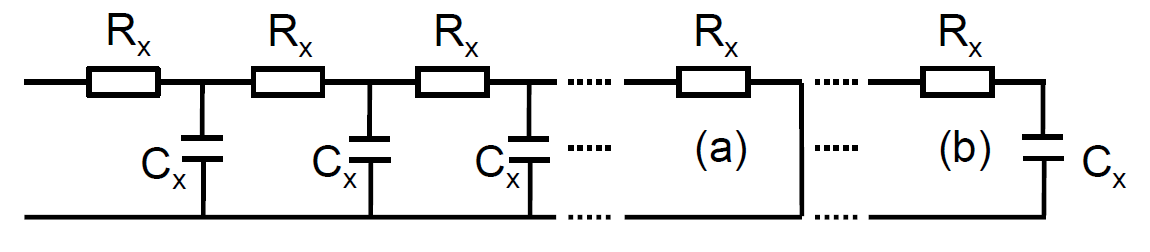
\includegraphics[width=0.9\columnwidth]{images/warburg_element.png}
	\caption{Kettenleitermodell eines Finite-Length (a) und Finite-Space (b) Warburg-Elements}
	\label{warburg_element}
\end{figure}
Das Impedanzspektrum einer Batterie kann mit Hilfe eines elektrochemischen Ersatzschaltbildes analysiert werden. Dabei versucht man für ein experimentell erhaltenes Impedanzspektrum ein plausibles Ersatzschaltbild zu finden, dessen Impedanzspektrum vom experimentell bestimmte Spektrum möglichst wenig abweicht. Ein Beispiel hierfür lässt sich in Abbildung \ref{schema_is} finden.
\\\\
Aus dem so modellierten Ersatzschaltbild lassen sich quantitative Aussagen über die einzelnen Widerstände und Grenzschichten innerhalb einer Batteriezelle treffen. Das Impedanzspektrum ist bei einer Batterie jedoch auch immer von Faktoren wie dem Ladezustand, der Temperatur oder der Anzahl an bereits erfolgter Zyklen abhängig.
\begin{figure}
	\centering
	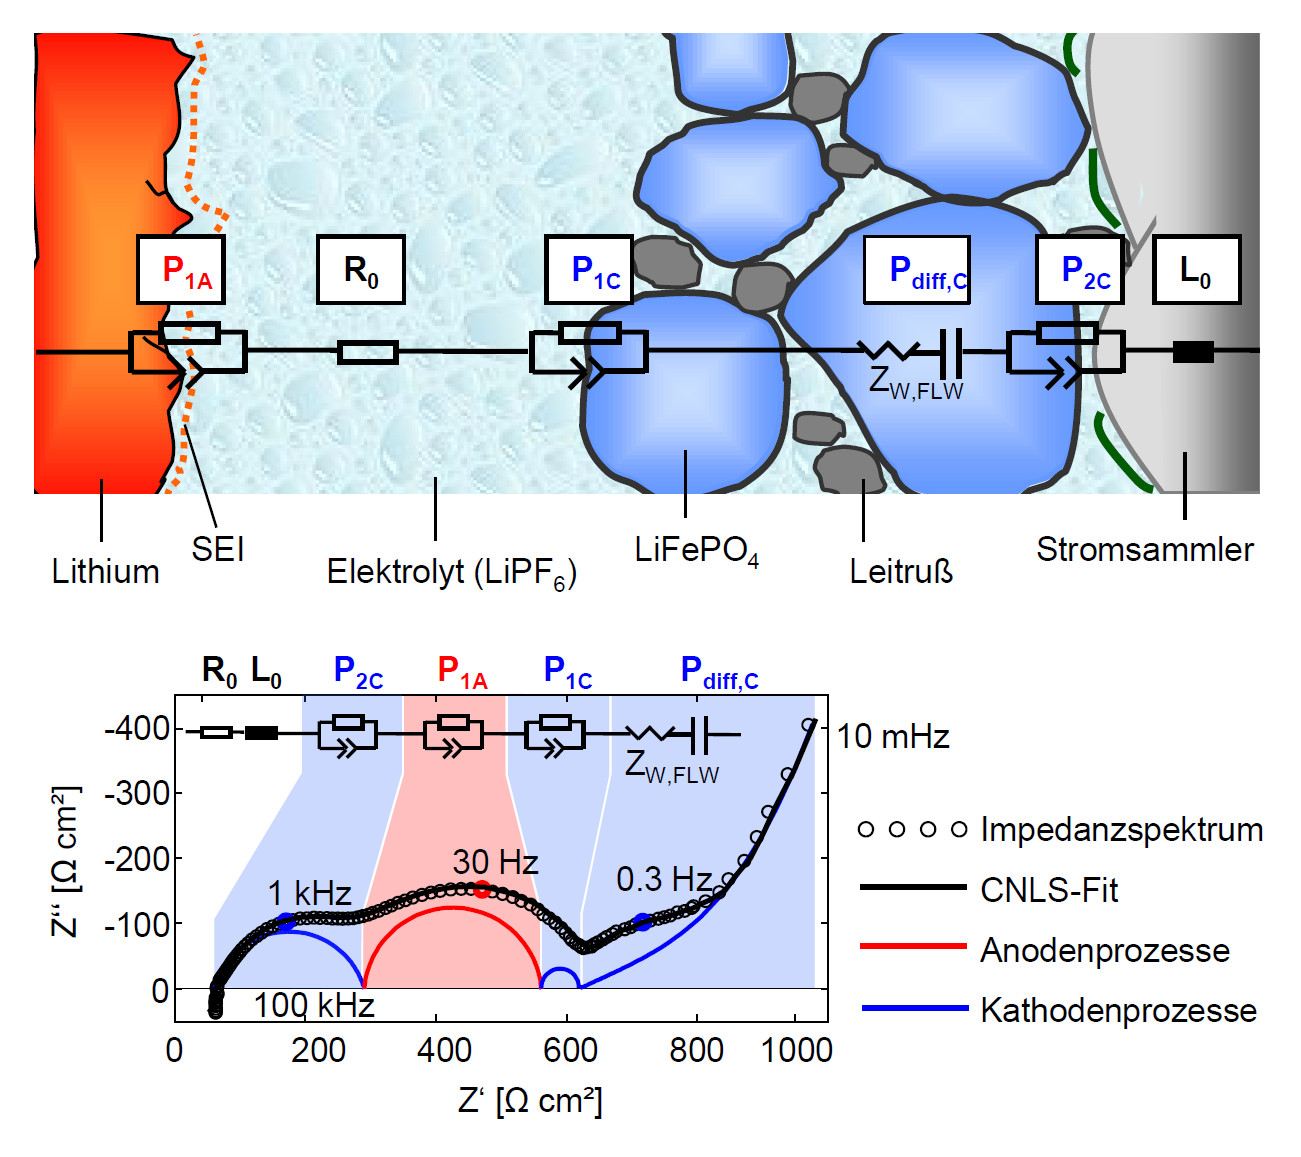
\includegraphics[width=0.8\columnwidth]{images/Schema_IS.jpg}
	\caption{Elektrochemisches Ersatzschaltbild und resultierendes Impedanzspektrum in Nyquist-Darstellung einer Li-\ce{LiFePO4}-Zelle}
	\label{schema_is}
\end{figure}
\subsection{Kernspinresonanzspektroskopie}
Die Grundlage der Kernspinresonanzspektroskopie (nuclear magnetic resonance spectroscopy, NMR-Spektroskopie) wurde zum Jahreswechsel 1945/1946 von zwei amerikanischen Forschungsgruppen unabhängig voneinander entwickelt. Felix Bloch und Edward M. Purcell wurden dafür 1952 mit dem Nobelpreis in Physik ausgezeichnet.
\subsubsection{Physikalische Grundlagen der NMR-Spektroskopie}
Die NMR-Spektroskopie nutzt die magnetischen Eigenschaften von Atomkernen und ihren Umgebungen aus, um Aussagen über Zusammensetzungen und Bindungen von Stoffen treffen zu können.
\\\\
Elektronen, Neutronen und Protonen besitzen eine Eigenrotation, den Spin s. Der Spin eines Atomkerns setzt sich aus den Spins der einzelnen Protonen und Neutronen innerhalb des Kerns zusammen. Spins sind gequantelt und können daher nur gewisse diskrete Zustände annehmen. Dies gilt auch für den resultierenden Gesamtspin des Atomkerns. Die möglichen Zustände des Kernspins eines spezifischen Isotops können beschrieben werden über seine Spinquantenzahl I. Es existieren folgende magnetische Spinquantenzahlen m, welche die möglichen Orientierungen des Spins beschreiben:
\begin{equation}
m_I = I, I-1, I-2, ..., -I
\end{equation}
Die Gesamtzahl an möglichen Zuständen entspricht daher der Summe von 2I+1. Das Li$^7$ besitzt die Spinquantenzahl I=$\frac{3}{2}$. Es gilt daher:
\begin{equation}
m_{I=\frac{3}{2}} = \frac{3}{2}, \frac{1}{2}, -\frac{1}{2}, -\frac{3}{2}
\end{equation}
Sind in einem Atomkern die Anzahl an Protonen und Neutronen beide gerade, so gilt für die Spinquantenzahl I=0. Ein solcher Nukleus besitzt keinen Kernspin und kann daher nicht mittels NMR-Spektroskopie untersucht werden.
\\\\
Ein Atomkern besitzt eine Ladung. Wenn diese durch einen Kernspin bewegt wird, so besitzt der Nukleus ein magnetisches Moment $\mu$ in Abhängigkeit zum Zustand des Spins. Der Zusammenhang zwischen einem Drehmoment P und dem magnetischen Moment kann allgemein über das gyromagnetische Verhältnis $\gamma$ beschrieben werden: 
\begin{equation}
\mu = \gamma P
\end{equation}
Das Drehmoment des Kerns in Richtung z eines frei gewählten kartesischen Koordinatensystems entspricht dabei seiner magnetischen Spinquantenzahl multipliziert mit dem reduzierten Planckschen Wirkungsquantum:
\begin{equation}
P_z = m_I \hbar
\label{magnMoment}
\end{equation}
Das magnetische Moment kann also beschrieben werden mit:
\begin{equation}
\mu_z = \gamma m_I \hbar
\end{equation}
Keiner dieser möglichen Spinzustände ist energetisch günstiger als die anderen. Die Zustände liegen daher degeneriert vor. Dies kann allerdings durch das Anlegen eines starken äußeren Magnetfeldes B$_0$ in positiver z-Richtung beeinflusst werden. Es bilden sich verschiedene Energieniveaus für die unterschiedlichen Spinzustände aus. Die Potentialenergie E kann beschrieben werden als:
\begin{equation}
E = -\mu_z B_0
\end{equation}
Mit Einsetzen von Gleichung \ref{magnMoment} ergibt sich daher mit den unterschiedlichen Spinorientierungen $m_I$:
\begin{equation}
E = -m_I \gamma \hbar B_0
\label{energiezustaende}
\end{equation}
Diese Aufspaltung der Energieniveaus ist bekannt als \textit{nuclear Zeeman splitting}. Die Energiedifferenz zwischen den Zuständen ist dabei proportional zur Stärke des angelegten äußeren Magnetfelds. Die Spins richten sich entlang der Achse aus. Die Energiedifferenzen sind dabei für jeden Kern, der einen Spin besitzt, charakteristisch und können mit einer Frequenz in Abhängigkeit zur Stärke des äußeren Magnetfelds beschrieben werden. Mit der \textit{Bohrschen Frequenzbedingung}:
\begin{equation}
\Delta E = hv
\end{equation}
kann die benötigte Quantenenergie bestimmt werden als: %gilt nur für den Protonenfall?
\begin{equation}
hv_0 = \gamma \hbar B_0
\end{equation}
Dargestellt als Frequenz:
\begin{equation}
\omega_0 = \gamma B_0
\end{equation}
Diese Frequenz wird als \textit{Larmor-Frequenz} bezeichnet und kann auch als Präzession des Kerns beschrieben werden. 
\\\\
Wird nun eine Transmitterspule in einem äußeren Magnetfeld $B_0$ mit einer spezifischen Larmor-Frequenz betrieben, so bringt sie exakt die nötige Energiedifferenz ein, um die Spins in einen energiereicheren Zustand zu promovieren. Das dadurch entstehende NMR-Signal kann mit einer Empfängerspule aufgezeichnet werden.
\\\\
Durch chemische Verbindungen entstehen um Atomkerne herum unterschiedlich dichte Elektronenwolken. Diese schirmen den Kern etwas vom äußeren Magnetfeld $B_0$ ab. Es entsteht ein lokales Magnetfeld $B_{lokal}$ um die Kerne herum, welches sich in seiner Stärke vom globalen Magnetfeld unterscheidet. Dadurch variiert die benötigte Anregungsfrequenz je nach der Umgebung eines Kernes leicht. Dieser Effekt findet sich als \textit{chemische Verschiebung} in Gestalt von unterschiedlichen Peaks im NMR-Spektrum wieder. Mit ihr ist es möglich Strukturaussagen über ein untersuchtes Material zu treffen.
\subsubsection{Aufbau eines NMR-Spektrometers}
\begin{figure}
	\centering
	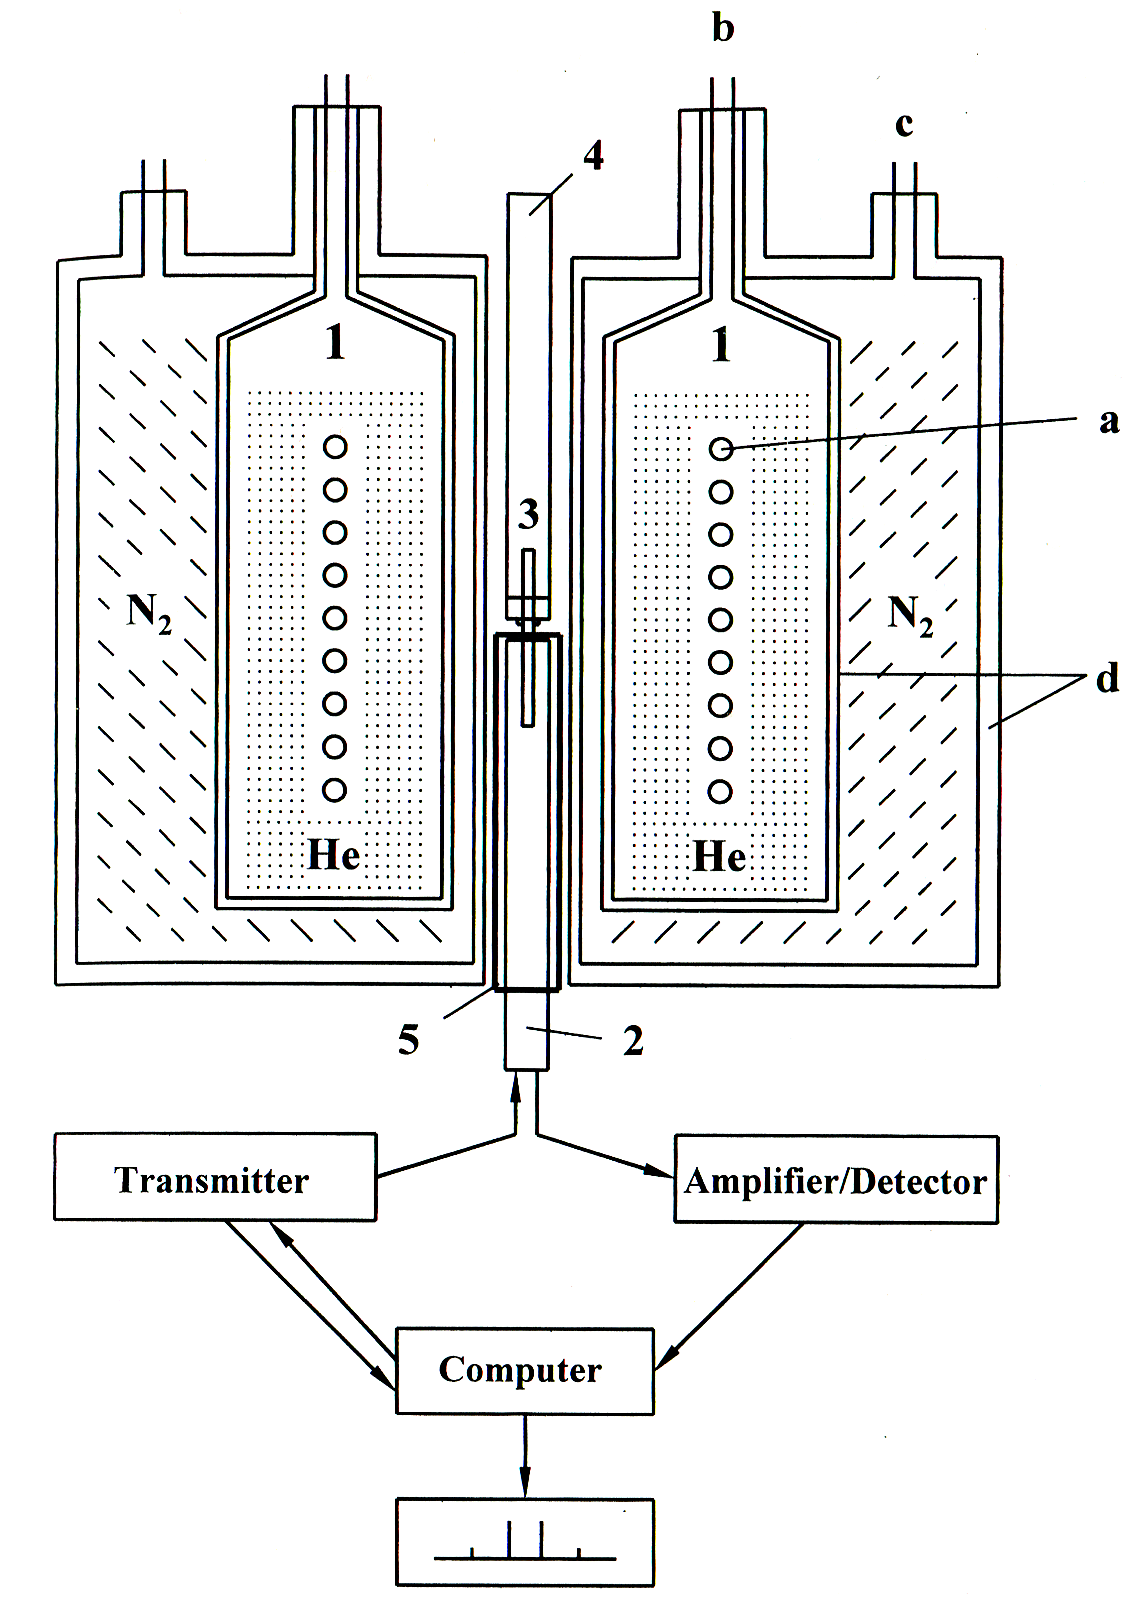
\includegraphics[width=0.9\columnwidth]{images/Aufbau_NMR.png}
	\caption{Schematischer Aufbau eines NMR-Spektrometers. Der Kryomagnetaufbau (1) mit Spule (a), Einfüllstutzen (b, c) und Vakuummänteln (d), Probenkopf (2), Probe (3), Probenwechsler (4) sowie Shim-Einheit (5). }
	\label{aufbau_nmr}
\end{figure}
Aus Gleichung \ref{energiezustaende} wird klar, dass die Größe der Potentialdifferenz zwischen energiereichen und -armen Zuständen mit der Stärke des Magnetfelds $B_0$ ansteigt. Die Kerne liegen dabei in Abhängigkeit zur Energiedifferenz $\Delta E$ boltzmannverteilt im energiereichen und -armen Zustand vor:
\begin{equation} %auch hier: Hinterer Teil gilt nur für den Protonenfall
\frac{N_{reich}}{N_{arm}} = \exp{\frac{-\Delta E}{kT}}=\exp{\frac{-\gamma h B_0}{2\pi k T}} \approx 1-\frac{\gamma h B_0}{2 \pi k T}
\end{equation}
Im Falle von H$^1$-NMR liegt die Energiedifferenz bei 0.04 J/mol. Bei Raumtemperatur und einer Magnetfeldstärke von 2,35 T ergibt sich damit eine Übergangswahrscheinlichkeit in den energiereichen Zustand von nur 0,002 \%. Um eine ausreichend gute Sensitivität zu gewährleisten, ist daher ein sehr starkes äußeres Magnetfeld $B_0$ nötig. Dies ist lediglich mit Kryomagneten zu erreichen.
\\\\
Der schematische Aufbau eines NMR-Spektrometers wird in Abbildung \ref{aufbau_nmr} dargestellt. Der Kryomagnetaufbau (1) besteht aus den Spulen (a), welche mit Flüssighelium gekühlt werden. Dieser wird wiederum mit Flüssigstickstoff umspült. Die Kühlflüssigkeiten können über spezielle Einlässe eingefüllt werden (b, c) und befinden sich in Vakuummänteln (d).
\\\\
 Der Probenkopf (2) wird von unten eingeführt und an eine Ansteuerungseinheit angeschlossen, welche die Transmitter- und die Empfängerspule ansteuert sowie das Signal aufzeichnet und ggf. verstärkt. Die Transmitter- und Empfängerspule kann meistens als eine Spule realisiert werden, welche beide Funktionen übernimmt. Sie ist im Probenkopf montiert, genauso wie die Entkoppler- Lock- und Gradientenspulen. Die Probe (3) wird von oben eingeführt, was durch einen Probenwechsler (4) passieren kann. Das äußere Magnetfeld $B_0$ liegt damit in Längsrichtung zur Probe. 
\\\\
Um die Feldhomogenität des eingepulsten Signals zu optimieren kann mit einer Shim-Einheit (5) ein \textit{Shimming} durchgeführt werden. Dieses besteht aus einem \textit{Tuning} und einem \textit{Matching}. Mit dem Tuning wird die durch die eingeführte Probe gedämpfte Empfindlichkeit des Probenkopfes auf die Resonanzfrequenz des zu untersuchenden Kerns eingestellt, um die höchstmögliche Empfindlichkeit zu gewährleisten. Das Matching besteht aus einer Impedanzanpassung, um die maximale Leistung am Probenkopf anliegen zu haben. Der gesamte Aufbau wird von einem Computer gesteuert und überwacht, welcher auch die Signalverarbeitung übernimmt.
\subsubsection{Betriebsmodus}
% Das hier ist schon arg rudimentär
% Beschreibung der Relaxationsmechanismen?
Es existieren zwei unterschiedliche Verfahren, um ein NMR-Spektrum zu messen. Das ältere von beiden ist das Continuous-Wave-Verfahren (CW). Beim CW-Verfahren wird eine monochromatische Strahlung in die Probe emittiert. Diese wird kontinuirlich variiert und die entsprechende Resonanz gemessen. Problematisch ist dabei vor allem die durch das Abfahren unterschiedlicher Frequenzen sehr lange Messzeit.
\\\\
Heute kommt nahezu ausschließlich das Puls-Fourier-Transform-Verfahren (PFT) zum Einsatz. Hierbei wird ein starker Frequenzpuls über einen Wellenlängenbereich auf die Probe abgegeben. Als Resonanz erhält man dabei einen \textit{Free Induction Decay} (FID), der als eine über den Zeitverlauf geschehende Einpendelbewegung in Larmor-Frequenz der angeregten Kerne beschrieben werden kann. Die sich dabei überlagernden Resonanzen können anschließend über eine Fourier-Transformation zum eigentlichen NMR-Spektrum zurückgerechnet werden.
\subsubsection{Magic Angle Spinning}
Festkörper haben im Vergleich zu Flüssigkeiten eine starrere Orientierung zu ihren Nachbarn und auch zum äußeren Magnetfeld $B_0$. Dies kann beispielsweise über die \textit{Dipolare Kopplung} eines Kerns zu einem magnetischen Moment $\mu$ in einer Entfernung $r$ unter einem Winkel $\theta$ gezeigt werden. Die Variation $\Delta B$ des lokalen Magnetfeld kann dann mit der Permeabilität des freien Raumes bestimmt werden zu:
\begin{equation}
\Delta B = \frac{\mu_0}{4\pi}(3\cos^2\theta - 1)\mu r
\end{equation}
Für Flüssigkeiten geht der Effekt der Diploaren Kopplung  durch thermische Bewegung und Rotation gegen Null, bei Feststoffen nicht. Er führt zu einer Verbreiterung der Peaks im Spektrum, was diese schwerer zu analysieren macht. Es gilt jedoch weiterhin:
\begin{equation}
3\cos^2\theta-1 = 0 \;\; \forall \;\; \theta = 54.7^\circ
\end{equation}
Dieser Winkel wird als \textit{magischer Winkel} (magic angle) bezeichnet. Wenn eine feste Probe also in einem speziellen Probengefäß (\textit{Spinner}) im magischen Winkel durch das Magnetfeld rotiert wird, so kann der Effekt der Dipolaren Kopplung auch bei Festkörpern verhindert werden. Diese Form der Kernspinresonanzspektroskopie nennt sich MAS-NMR.
\chapter{Methodik}
Zuerst wird die Herstellung unterschiedlicher keramischer Pulver beschrieben. Anschließend erfolgt die Beschreibung der Mischung zu Elektrodenslurries und des Foliengusses. Im dritten Abschnitt wird die Konstruktion und der Bau einer neuen in-situ NMR-Testzelle beschrieben. Im letzten Abschnitt wird der Bau der unterschiedlichen Batterie-Testzellen dargestellt. 
\section{Pulverherstellung}
Es wurden zwei Pulver selbst hergestellt. Weitere bereits am Institut vorhandene und charakterisierte Pulver wurden für die darauf folgenden Schritte ausgewählt.
\subsection{LATP}
Bei der Herstellung des LATP kommt das Sol-Gel-Verfahren zum Einsatz. Als Ausgangsmaterial werden drei Stoffe verwendet: Aluminiumnitrat (\ce{Al(No3)3 \; 9H2O}, Aluminiumnitrate nonahydrat, EMSURE), Lithiumacetat (\ce{LiOOCH3 \; 2H2O} Lithiumacetate dihydrate, Reagent Grade, Alfa Aesar) und Tetra\-iso\-propyl\-ortho\-titanat (\ce{C12H28O4Ti}, Merck). Die Einwaage der Stoffe erfolgt stöchiometrisch. Alle werden jeweils in Wasser gelöst und anschließend miteinander vermengt. Danach wird Phosphorsäure (\ce{H3PO4}) zugegeben. Auf Grund der dabei entstehenden Reaktionswärme erfolgt dies in einem Wasserbad unter kontinuierlichen Rühren.
\\\\
Um die organischen Anteile des Gels zu entfernen, wird dieses zunächst für acht Stunden bei 400$^\circ$C wärmebehandelt. In einem zweiten Schritt kann dann mit einem weiteren Glühschritt bei 900$^\circ$C für acht Stunden die gewünschte LATP-Struktur erzeugt werden. Um feinere Agglomerate zu erhalten wird das Pulver noch mit einem Mörser zerkleinert.
\subsection{\ce{LiTiPO5}}
\begin{figure}
	\centering
	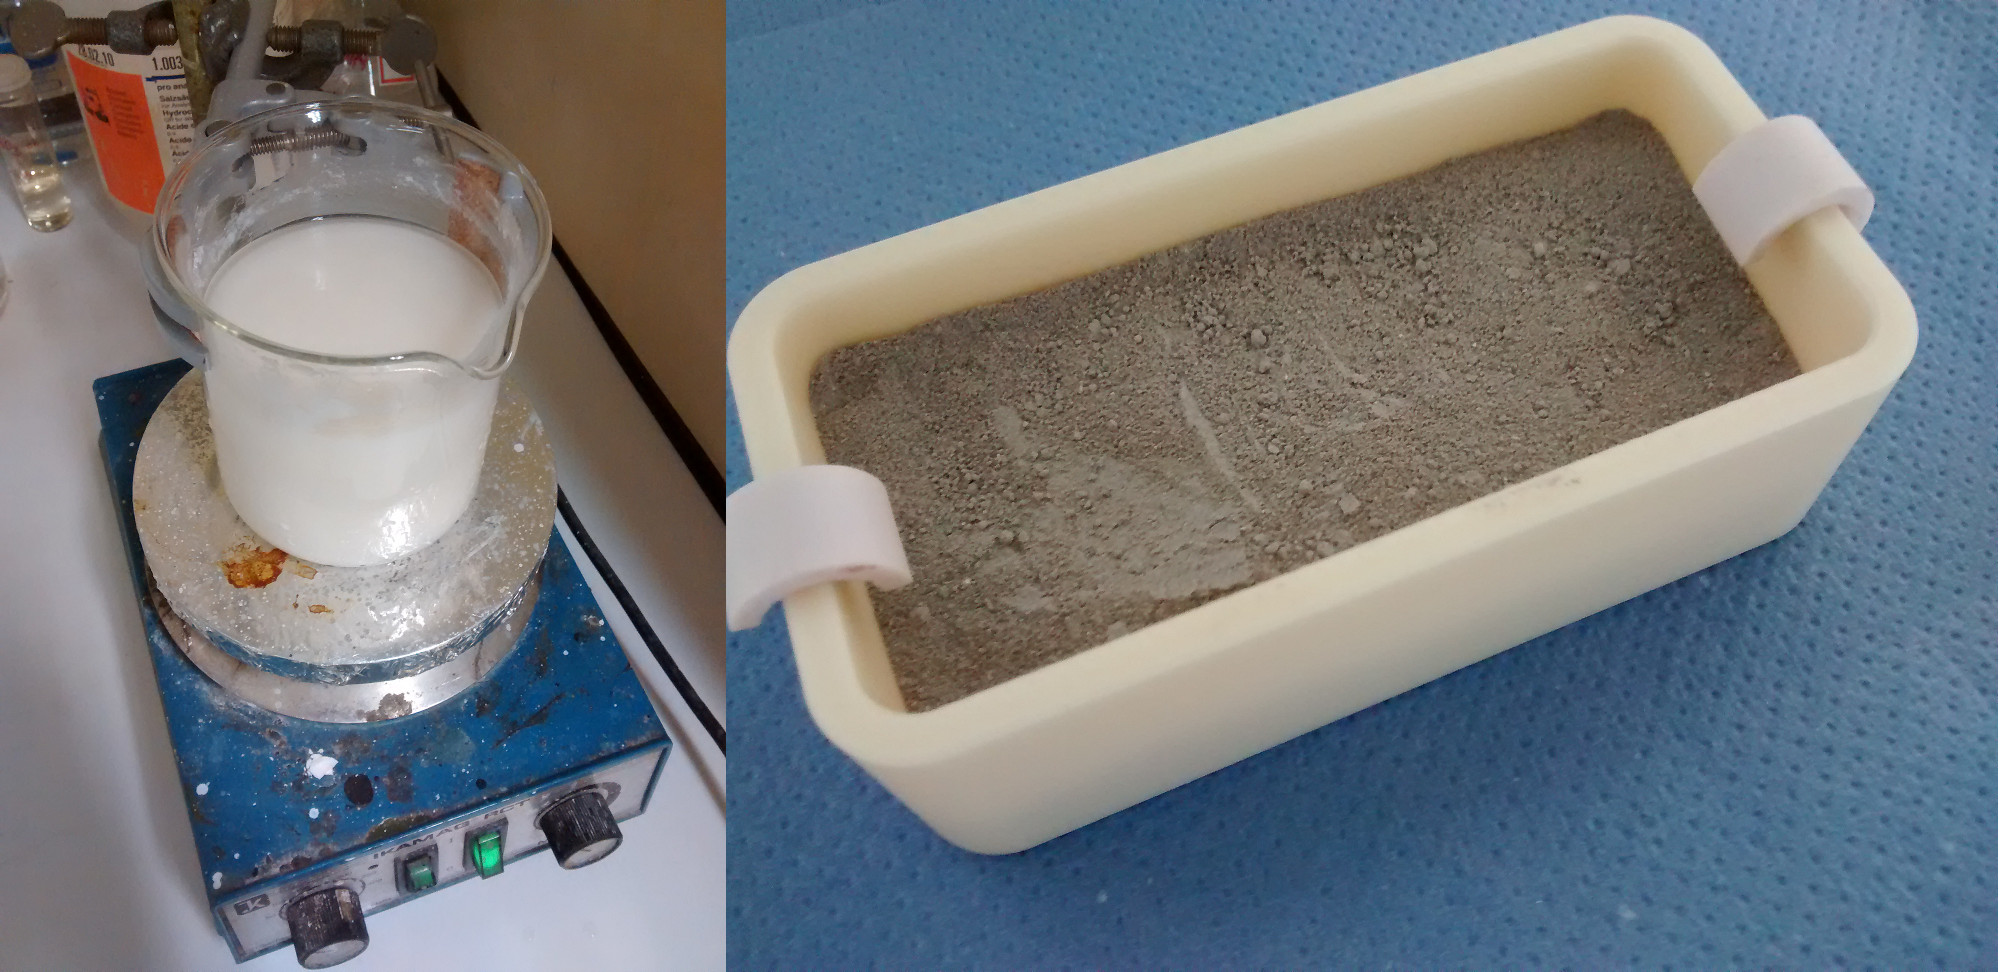
\includegraphics[width=1.0\columnwidth]{images/SolGel.jpg}
	\caption{Herstellung von \ce{LiTiPO5} über einen Sol-Gel-Prozess}
	\label{sol_gel}
\end{figure}
Die Herstellung des \ce{LiTiPO5} erfolgt analog zur Herstellung des LATP im Sol-Gel-Verfahren. Es wird jedoch auf das Aluminiumnitrat verzichtet.
\\\\
Zur Befreiung des Gels von unerwünschten organischen Bestandteilen wird dieses für acht Stunden bei 400$^\circ$C ausgebrannt. Anschließend erfolgt eine Wärmebehandlung bei 900$^\circ$C. Abschließend wird das Pulver noch mit einem Mörser zerkleinert. Abbildung \ref{sol_gel} zeigt die Herstellung des Gels sowie das Pulver nach dem Ausbrennen.
\subsection{Weitere verwendete Pulver}
\label{methodik_weitere_Pulver}
Drei weitere bereits am Institut hergestellte und charakterisierte Pulver wurden zur weiteren Untersuchung mittels MAS-NMR und zur Weiterverarbeitung zu Elektrodenslurries ausgewählt.  
% Hinweis auf Paul?
\subsubsection{LAGP}
Die Herstellung von LAGP erfolgt ebenfalls über den Sol-Gel-Prozess, der auch schon bei LATP angewendet wurde. Anstatt Titanphosphat wird Germaniumoxid ($>99\%$, Aldrich) verwendet. Dieses bildet mit Wasser allerdings keine homogene Lösung, weshalb der Ansatz mittels kontinuierlichem Rühren am Sedimentieren gehindert werden muss. Überschüssiges Wasser wird noch vor dem Kalzinierschritt verdampft.
\\\\
Charakterisierung, XRD
\subsubsection{LLTO}
Bei der Herstellung des LLTO kommt ein Mischoxid-Prozess zum Einsatz. Lithiumcarbonat (\ce{Li2CO3}, 99,998\%, Alfa Aesar) und Titandioxid (\ce{TiO2}, Titanium(IV) oxide, $>99.9\%$, Aldrich) werden in Isopropanol dispergiert und in einem Attritor deagglomeriert sowie homogenisiert. Das Isopropanol wird mit einem Rotationsverdampfer und mit einer eintägigen Lagerung in einem Vakuumtrockenschrank bei 60$^\circ$C entfernt. Als letzter Schritt wird das Pulver bei 800$^\circ$C für 12 Stunden kalziniert.
\\\\
Charakterisierung, XRD
\subsubsection{LTO}
Die Herstellung von LTO erfolgt analog zu der des LLTO. Es wird jedoch noch zusätzlich Lanthanoxid (Lanthanum(III) oxide, 99,99\%, Aldrich) mit in Isopropanol dispergiert. Weiterhin wird ein Lanthanüberschuss von 2,5 m\% vorgelegt. Die Kalzinierung findet für acht Stunden bei 950$^\circ$C statt.
\\\\
Charakterisierung, XRD
\section{Elektrodenherstellung}
Die hergestellten und ausgewählten Pulver werden anschließend zu Elektroden weiterverarbeitet. Dazu müssen Elektrodenslurries hergestellt werden und auf Folien gegossen werden. Alternativ erfolgt die Sinterung eines Gefüges aus Elektrode und Elektrolyt.
\subsection{Herstellung verschiedener Elektrodenslurries}
Es wurden aus den keramischen Pulvern LATP, LAGP, LLTO und LTO  Elektrodenslurries hergestellt. Zusätzlich wurden aus den herkömmlichen Aktivmaterialien \ce{LiCoO2} und Schwefel Elektrodenslurries produziert. Dabei wurde jeweils der gleiche Prozess verwendet. 
\\\\
Zunächst wird das ausgewählte Pulver als Aktivmaterial in N-Methyl-2-pyrrolidon (NMP, \ce{C5H9NO}, 99,5\%, Alfa Aesar) gelöst. Anschließend wird masseäquivalent zum Aktivmaterial das Leitruß Super C65 (TIMCAI), falls nötig unter Zugabe von weiterem NMP, beigemengt. Das Gemisch wird mit einem Ultraschallstab homogenisiert. Dies geschieht wegen der Wärmeentwicklung im Wasserbad. Abschließend wird ein NMP-Binder-Gemisch (Masseverhältnis $19:1$) zugegeben. Als Binder kommt Solef PVDF (Polyvinylidenfluorid, \ce{C2H2F2}, Solvay) zum Einsatz. Der Anteil an Binder im Gesamtgewicht wird dabei auf 10m\% eingestellt. Da das PVDF durch eine Ultraschallbehandlung Schaden nehmen würde, erfolgt das Vermischen für eine Stunde mittels eines Rührfisches unter einer Vakuumglocke.
\subsection{Foliengießen der Elektroden}
Als Stromkollektor wird handelsübliche Aluminiumfolie zurechtgeschnitten. Diese wird mit der rauen Seite nach oben auf das Foliengussgerät AB3320 der Firma TQC aufgelegt. Dieses zieht die Folie mittels Vakuum an, ein händisches Glattstreichen verhindert Falten. Anschließend wird ein Aluminiumschuh auf die Folie aufgelegt. Dieser bestimmt die Schichtdicke der Elektrode über die Schlitzhöhe am Boden des Schuhs. Dicken über 300$\mu$m zeigten eine unzureichende Trocknung und Haftung, weshalb alle Folien mit einer Höhe von 200$\mu$m gegossen wurden.
\\\\
Die Folien werden anschließend zur Trocknung und Ausdampfung des NMP für mehrere Tage in einen Vakuumtrockenschrank bei 80$^\circ$C gelegt. Die fertigen Elektrodenfolien werden in Klarsichthüllen trocken gelagert.
\begin{figure}
	\centering
	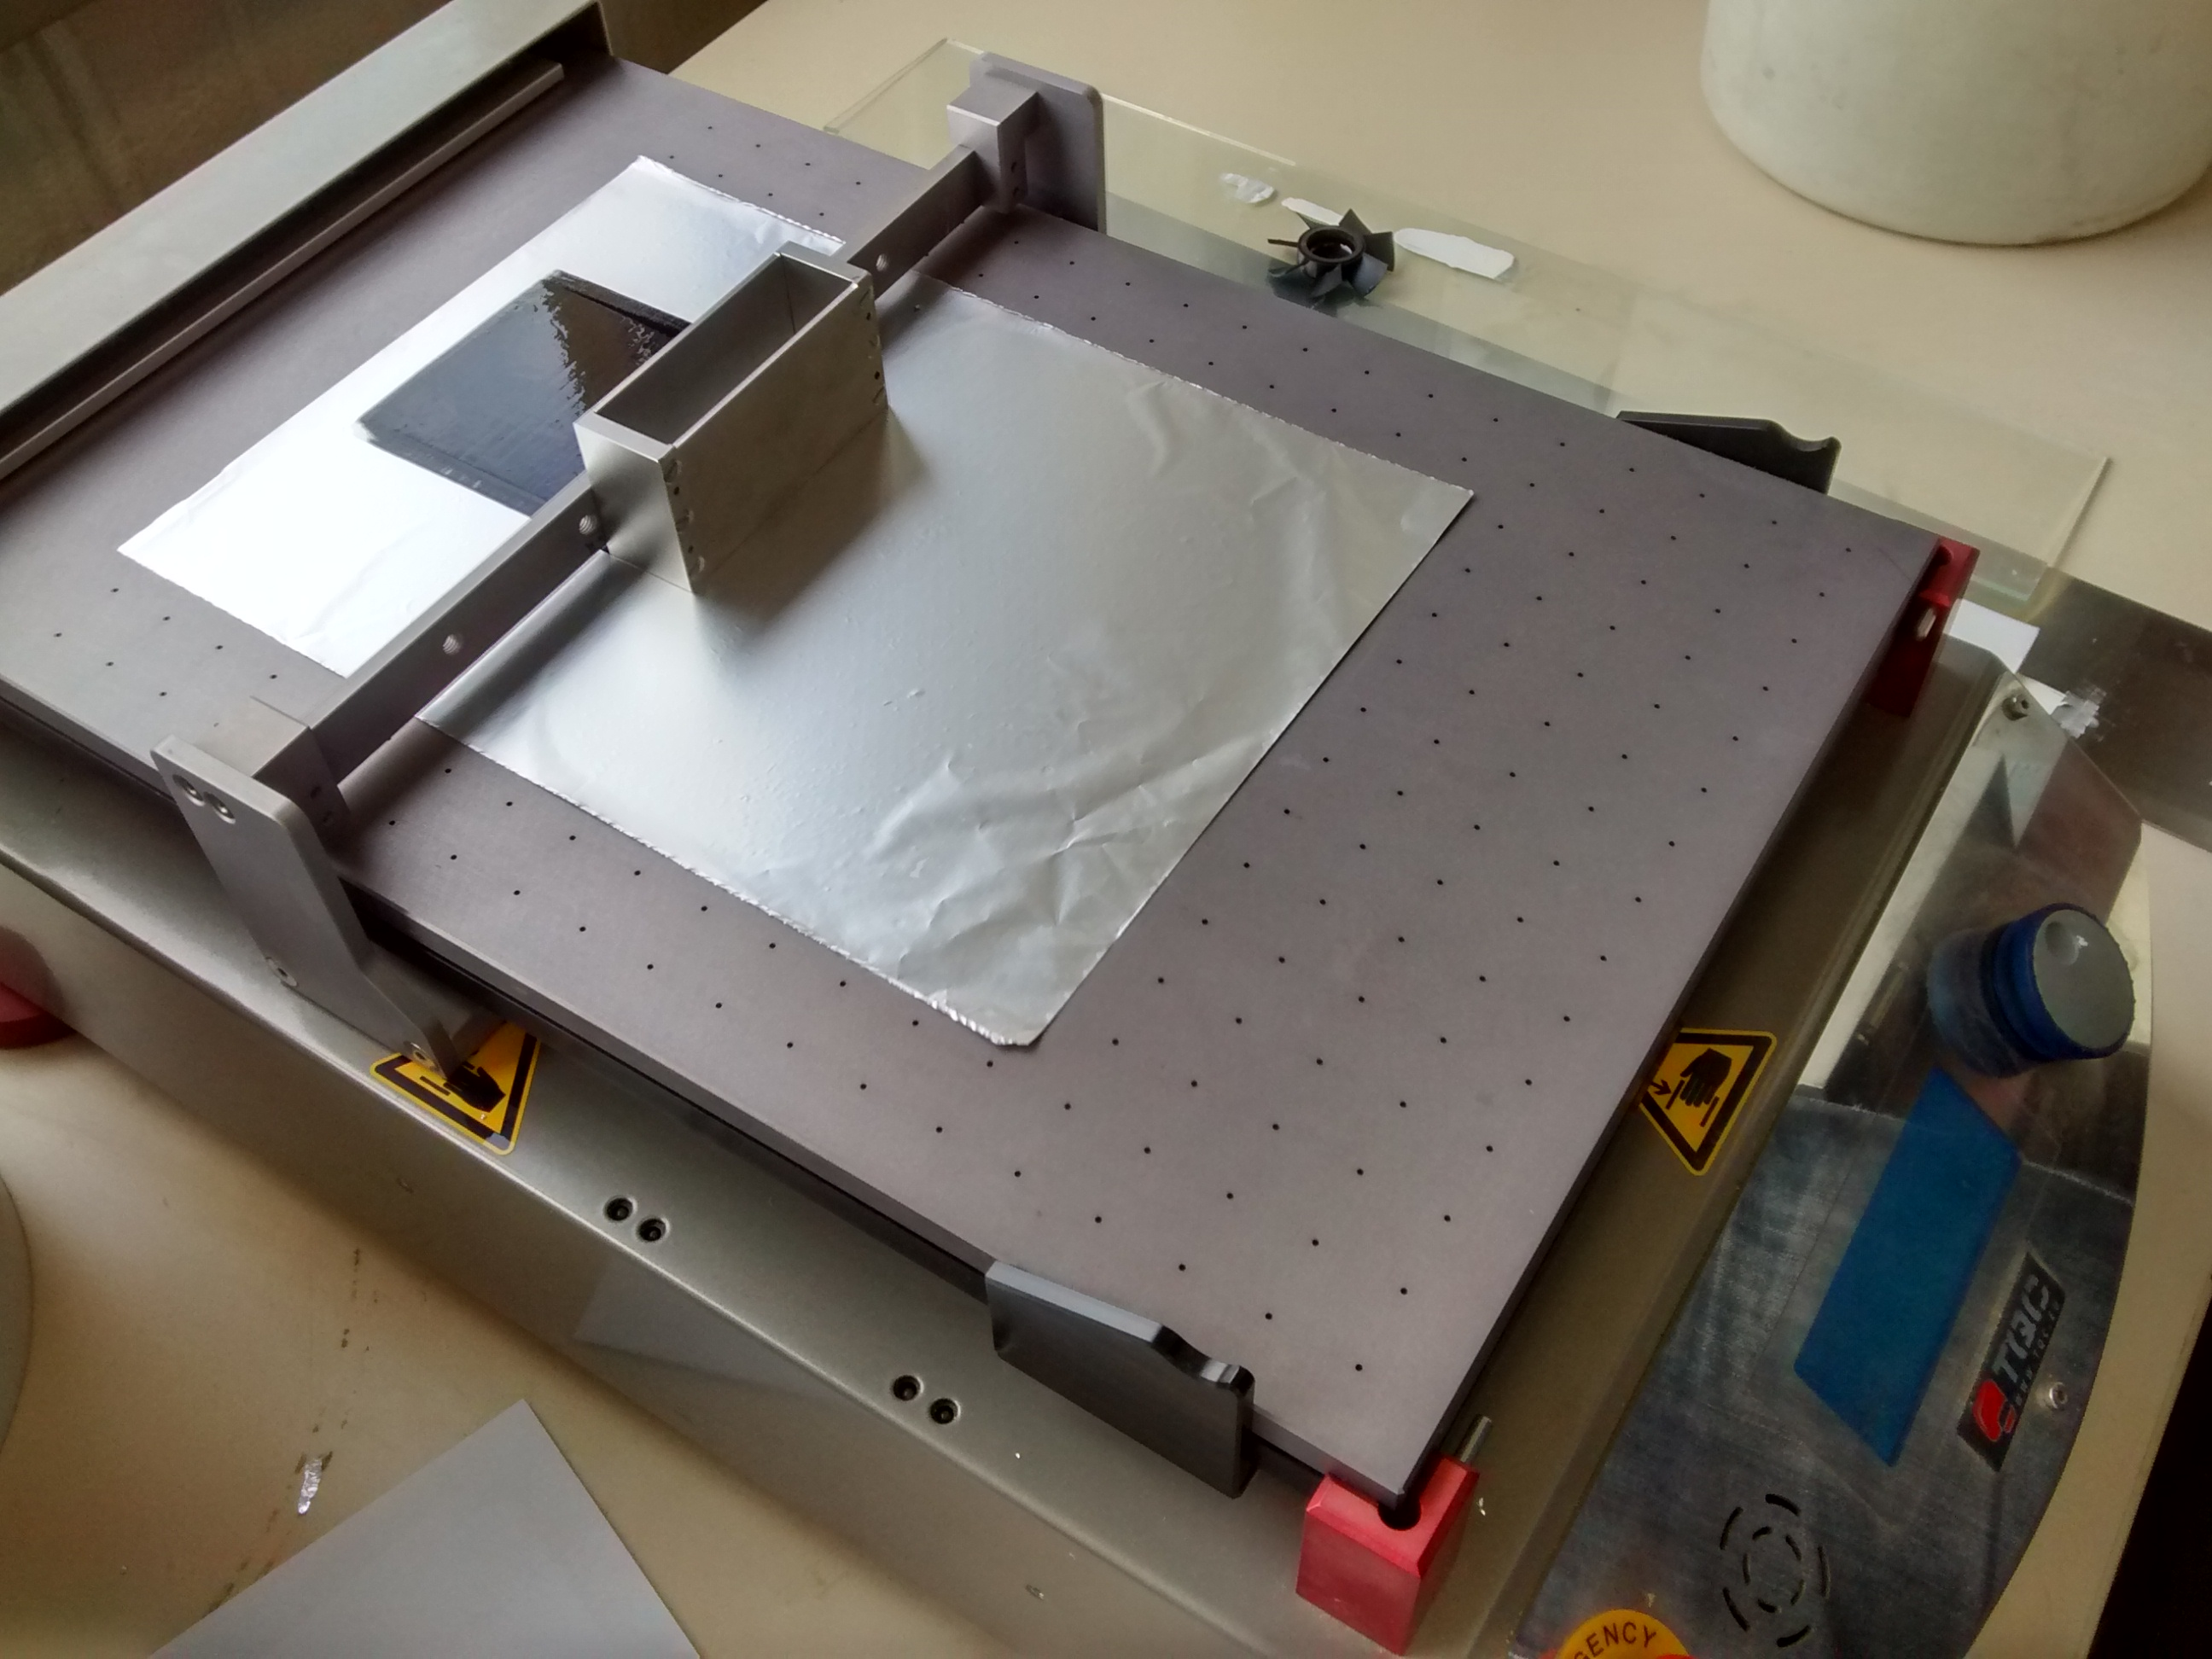
\includegraphics[width=0.85\columnwidth]{images/folienguss.jpg}
	\caption{Folienguss einer Elektrode auf Aluminiumfolie}
	\label{folienguss}
\end{figure}
\subsection{Herstellung eines Elektrode-Elektrolyt-Gefüges}
Für die Herstellung eines Elektrode-Elektrolyt-Gefüges wird zunächst 1,2g LTO in eine Matrize für das Spark-Plasma-Sintern (SPS) mit einem Durchmesser von 20mm verteilt. Darauf werden 1,5g LLTO aufgebracht. Die Pulver werden mit einer Handpresse mit 3kN vorgepresst. Anschließend wird die Matrize in die SPS-Anlage eingebaut. 
\\\\
Die SPS-Anlage legt nach Einbau erstmal einen Druck von 5kN auf die Matrize auf. Der Druck wird dann auf 7,8kN erhöht, bevor die Temperatur mit 50$^\circ$C/min auf 900$^\circ$C angepasst wird. Diese Temperatur wird eine Minute gehalten, bevor der Druck für fünf Minuten auf 15kN gesteigert wird. Anschließend wird die Probe bei 7,8kN abgekühlt. Eine Übersicht über den Prozess findet sich in Abbildung (noch einfügen).
\section{Anpassung des NMR-Probenkopfes}
\begin{figure}
	\centering
	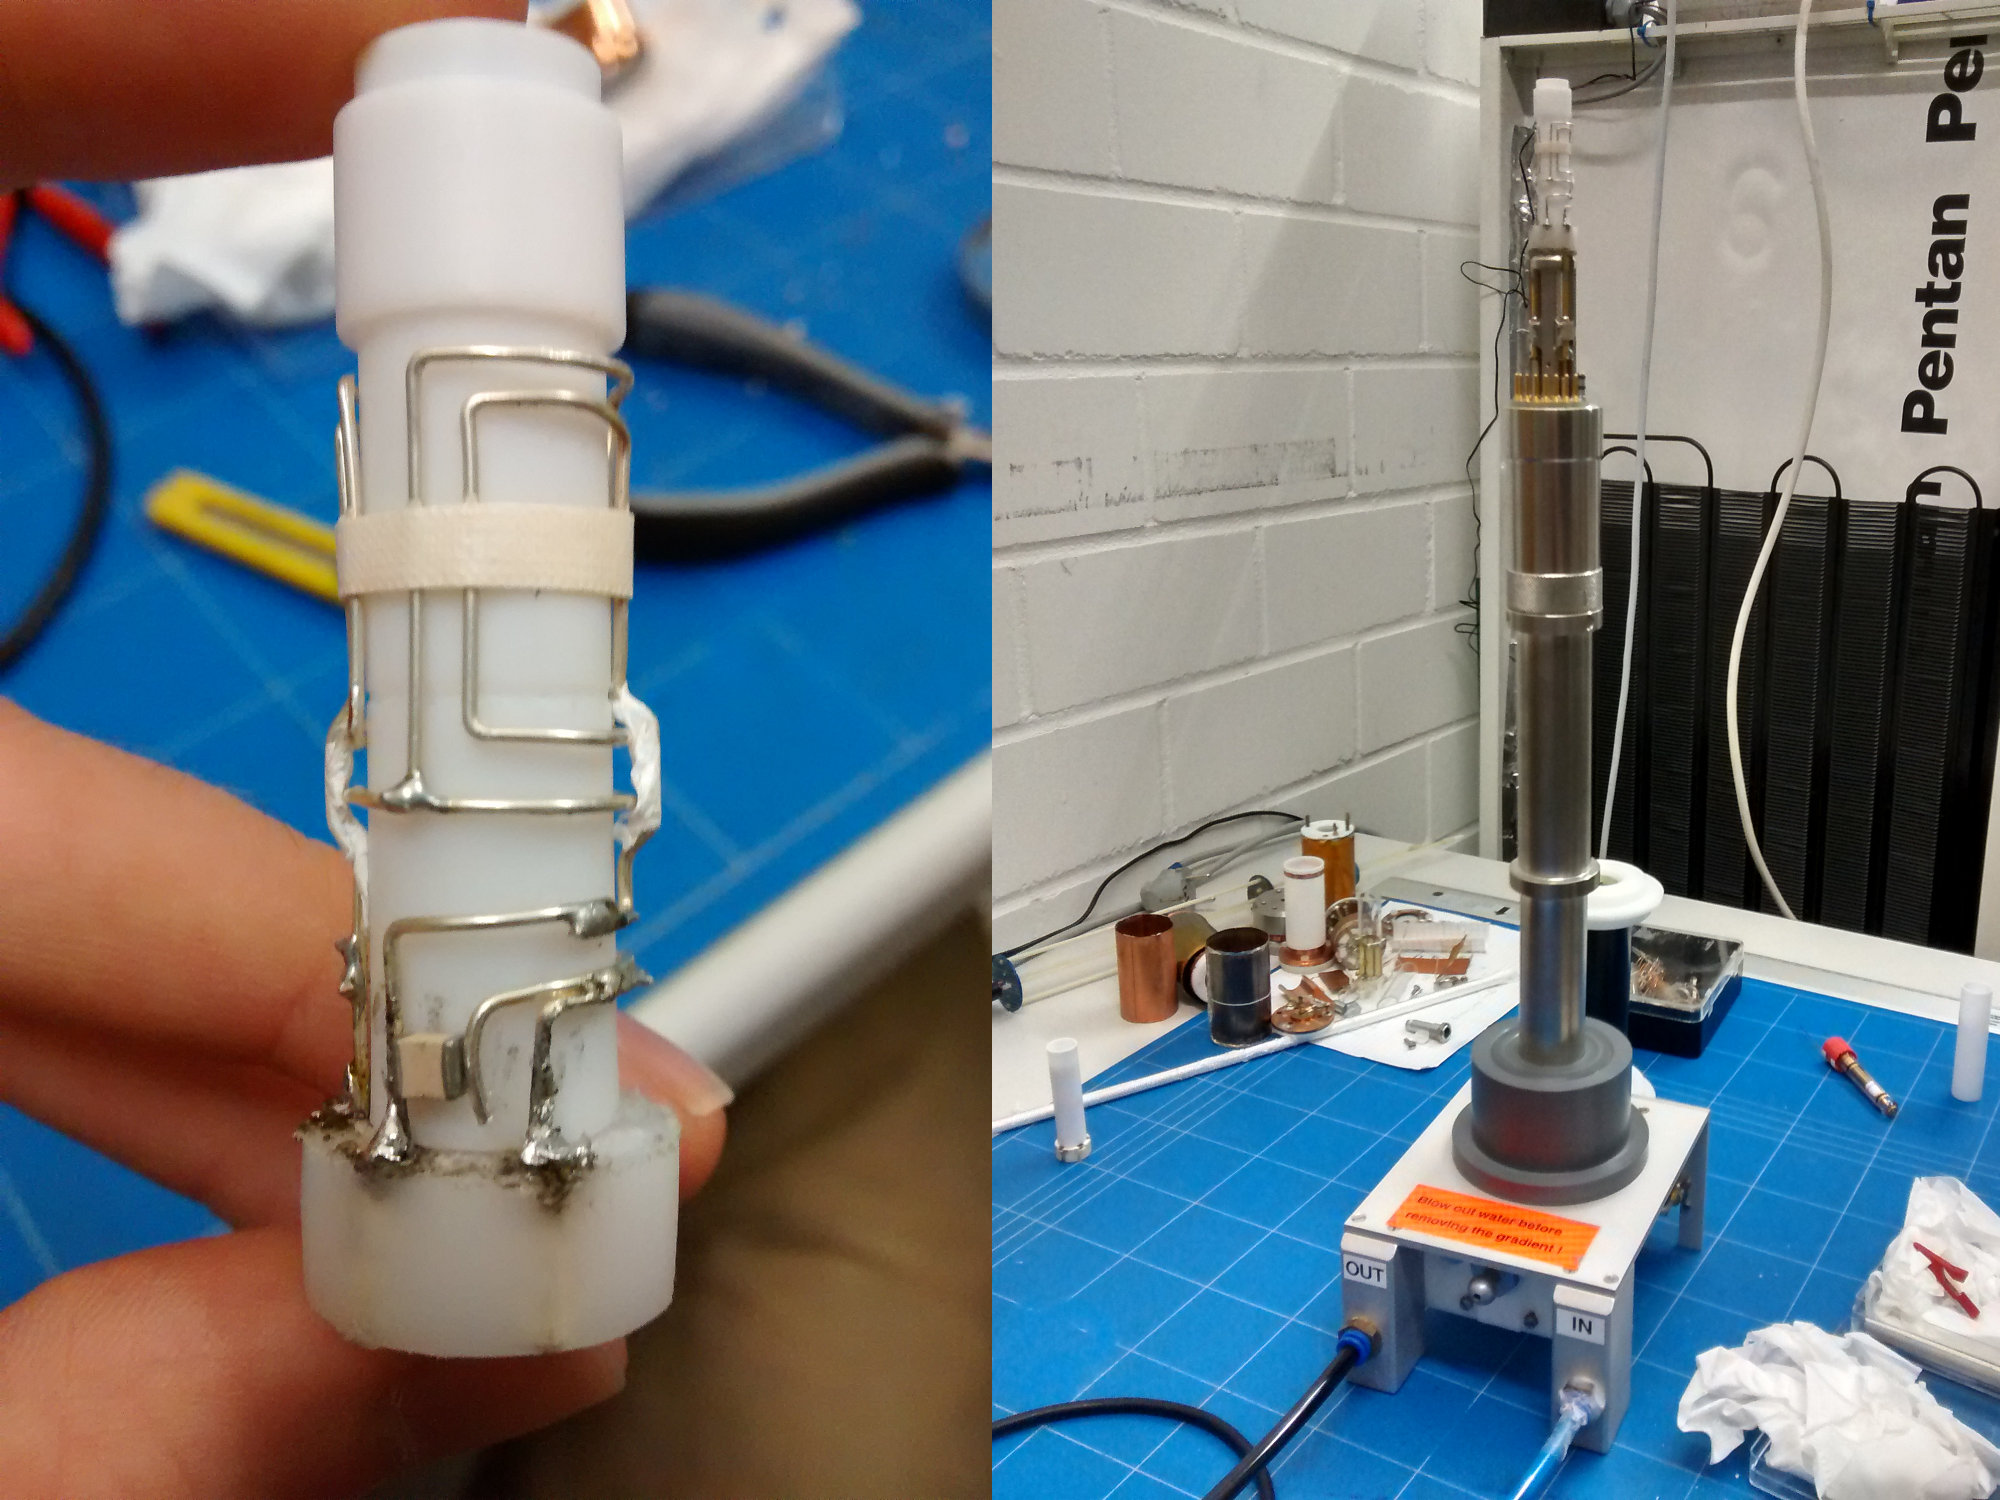
\includegraphics[width=0.85\columnwidth]{images/Platzhalter_Spule.jpg}
	\caption{Spule mit Kondensator (links) und eingebaut in den Probenkopf (rechts)}
	\label{spule}
\end{figure}
Die in-situ-Testzelle kommt im 200MHz-NMR-Spektrometer der Firma mBruker am Institut XY zum Einsatz. Dafür wurde der Probenkopf entsprechend angepasst. Es wurde eine neue Sattelspule um ein Teflonrohr mit Innendurchmesser von 10mm gewickelt. Diese musste anschließend mit dem Anschlussstempel des Probenkopfes verlötet werden. Damit die Spule auf der richtigen Resonanzfrequenz von 77,7MHz für Li$^7$-NMR arbeitet, wurde ein 5pF-Kondensator in den Spulen-Schwingkreis eingebaut. Um einen Kurzschluss der Spule durch die massive Kupferabschirmung nach außen hin zu vermeiden, wird eine zweite Teflonröhre über die Spule gestülpt.
\section{Konstruktion der in-situ-Testzelle}
Um NMR-Messungen im laufenden Betrieb einer Batterie machen zu können, musste ein spezieller Testaufbau geplant und kostruiert werden. Es war nötig sowohl den Probenkopf des NMR-Spektrometers anzupassen, als auch eine komplett neue Batterie-Testzelle zu bauen.
\subsection{Anforderungen}
Ziel ist die Konstruktion einer Testzelle, in welcher sowohl herkömmliche Batterien als auch Festkörperelektrolyt-Batterien eingebaut werden können. Für den Einsatz von reinem Lithium\-metall und Flüssigelektrolyten muss die Testzelle gasdicht gebaut werden können. Die eingesetzten Materialien müssen alle ausreichend amagnetisch sein, um die empfindlichen Kernspinresonanzmessungen der NMR-Spektroskopie nicht zu sehr zu stören. Sie sollte möglichst ähnlich wie die bereits am IAM-KWT im Einsatz befindliche Zelle aufgebaut sein, um eine Vergleichbarkeit zwischen beiden Zellen zu gewährleisten und einen Einsatz auch außerhalb der NMR-Anlage zu ermöglichen. 
\\\\
Der Außendurchmesser der Zelle ist durch den Aufbau des NMR-Probenkopfes auf maximal 10mm festgesetzt. Eine Ausnahme stellt hier der Zellabschluss dar, da dieser über die Teflonhülle der Spule des Probenkopfes reichen kann und daher lediglich durch die Öffnung der Kupferabschirmung des Probenkopfes beschränkt ist. Diese hat einen Durchmesser von 16,5mm. Der relevante Messbereich der Spule befindet sich auf einer Höhe von 22mm bis 32mm. Ein Anschluss an den externen Stromkreis zum Laden und Entladen der Zelle kann nur nach oben hin erfolgen.
\\\\
In der Literatur lassen sich unterschiedliche Umsetzungen von in-situ-Testzellen für NMR-Spektroskopie finden. Die Arbeitsgruppe um Silvio Indris am IAM-ESS sowie Zhou et al. \cite{zhou2013paramagnetic} und Key et al. \cite{key2009real} benutzen dafür Pouch-Zellen, die gerollt oder gefaltet in den NMR-Aufbau eingebracht werden können. Dies ist jedoch mit Festkörperelektrolyten wegen des starren Aufbaus der Zelle nicht möglich, weshalb dieser Ansatz nicht verfolgt wurde.  Poli et al. \cite{poli2011new} und Gerald et al. \cite{gerald2001situ} implementieren beide einen Knopfzellenaufbau. Beide Lösungen sehen aber einen umfangreichen Umbau des NMR-Probenkopfes vor. Die angestrebte Lösung soll jedoch eine weitere Verwendung des Probenkopfes für andere NMR-Experimente im gewohnten Messaufbau und damit einhergehend schnelles Umrüsten des Probenkopfes ermöglichen.
\subsection{Planung und Anfertigung der Teile}
\begin{figure}
	\centering
	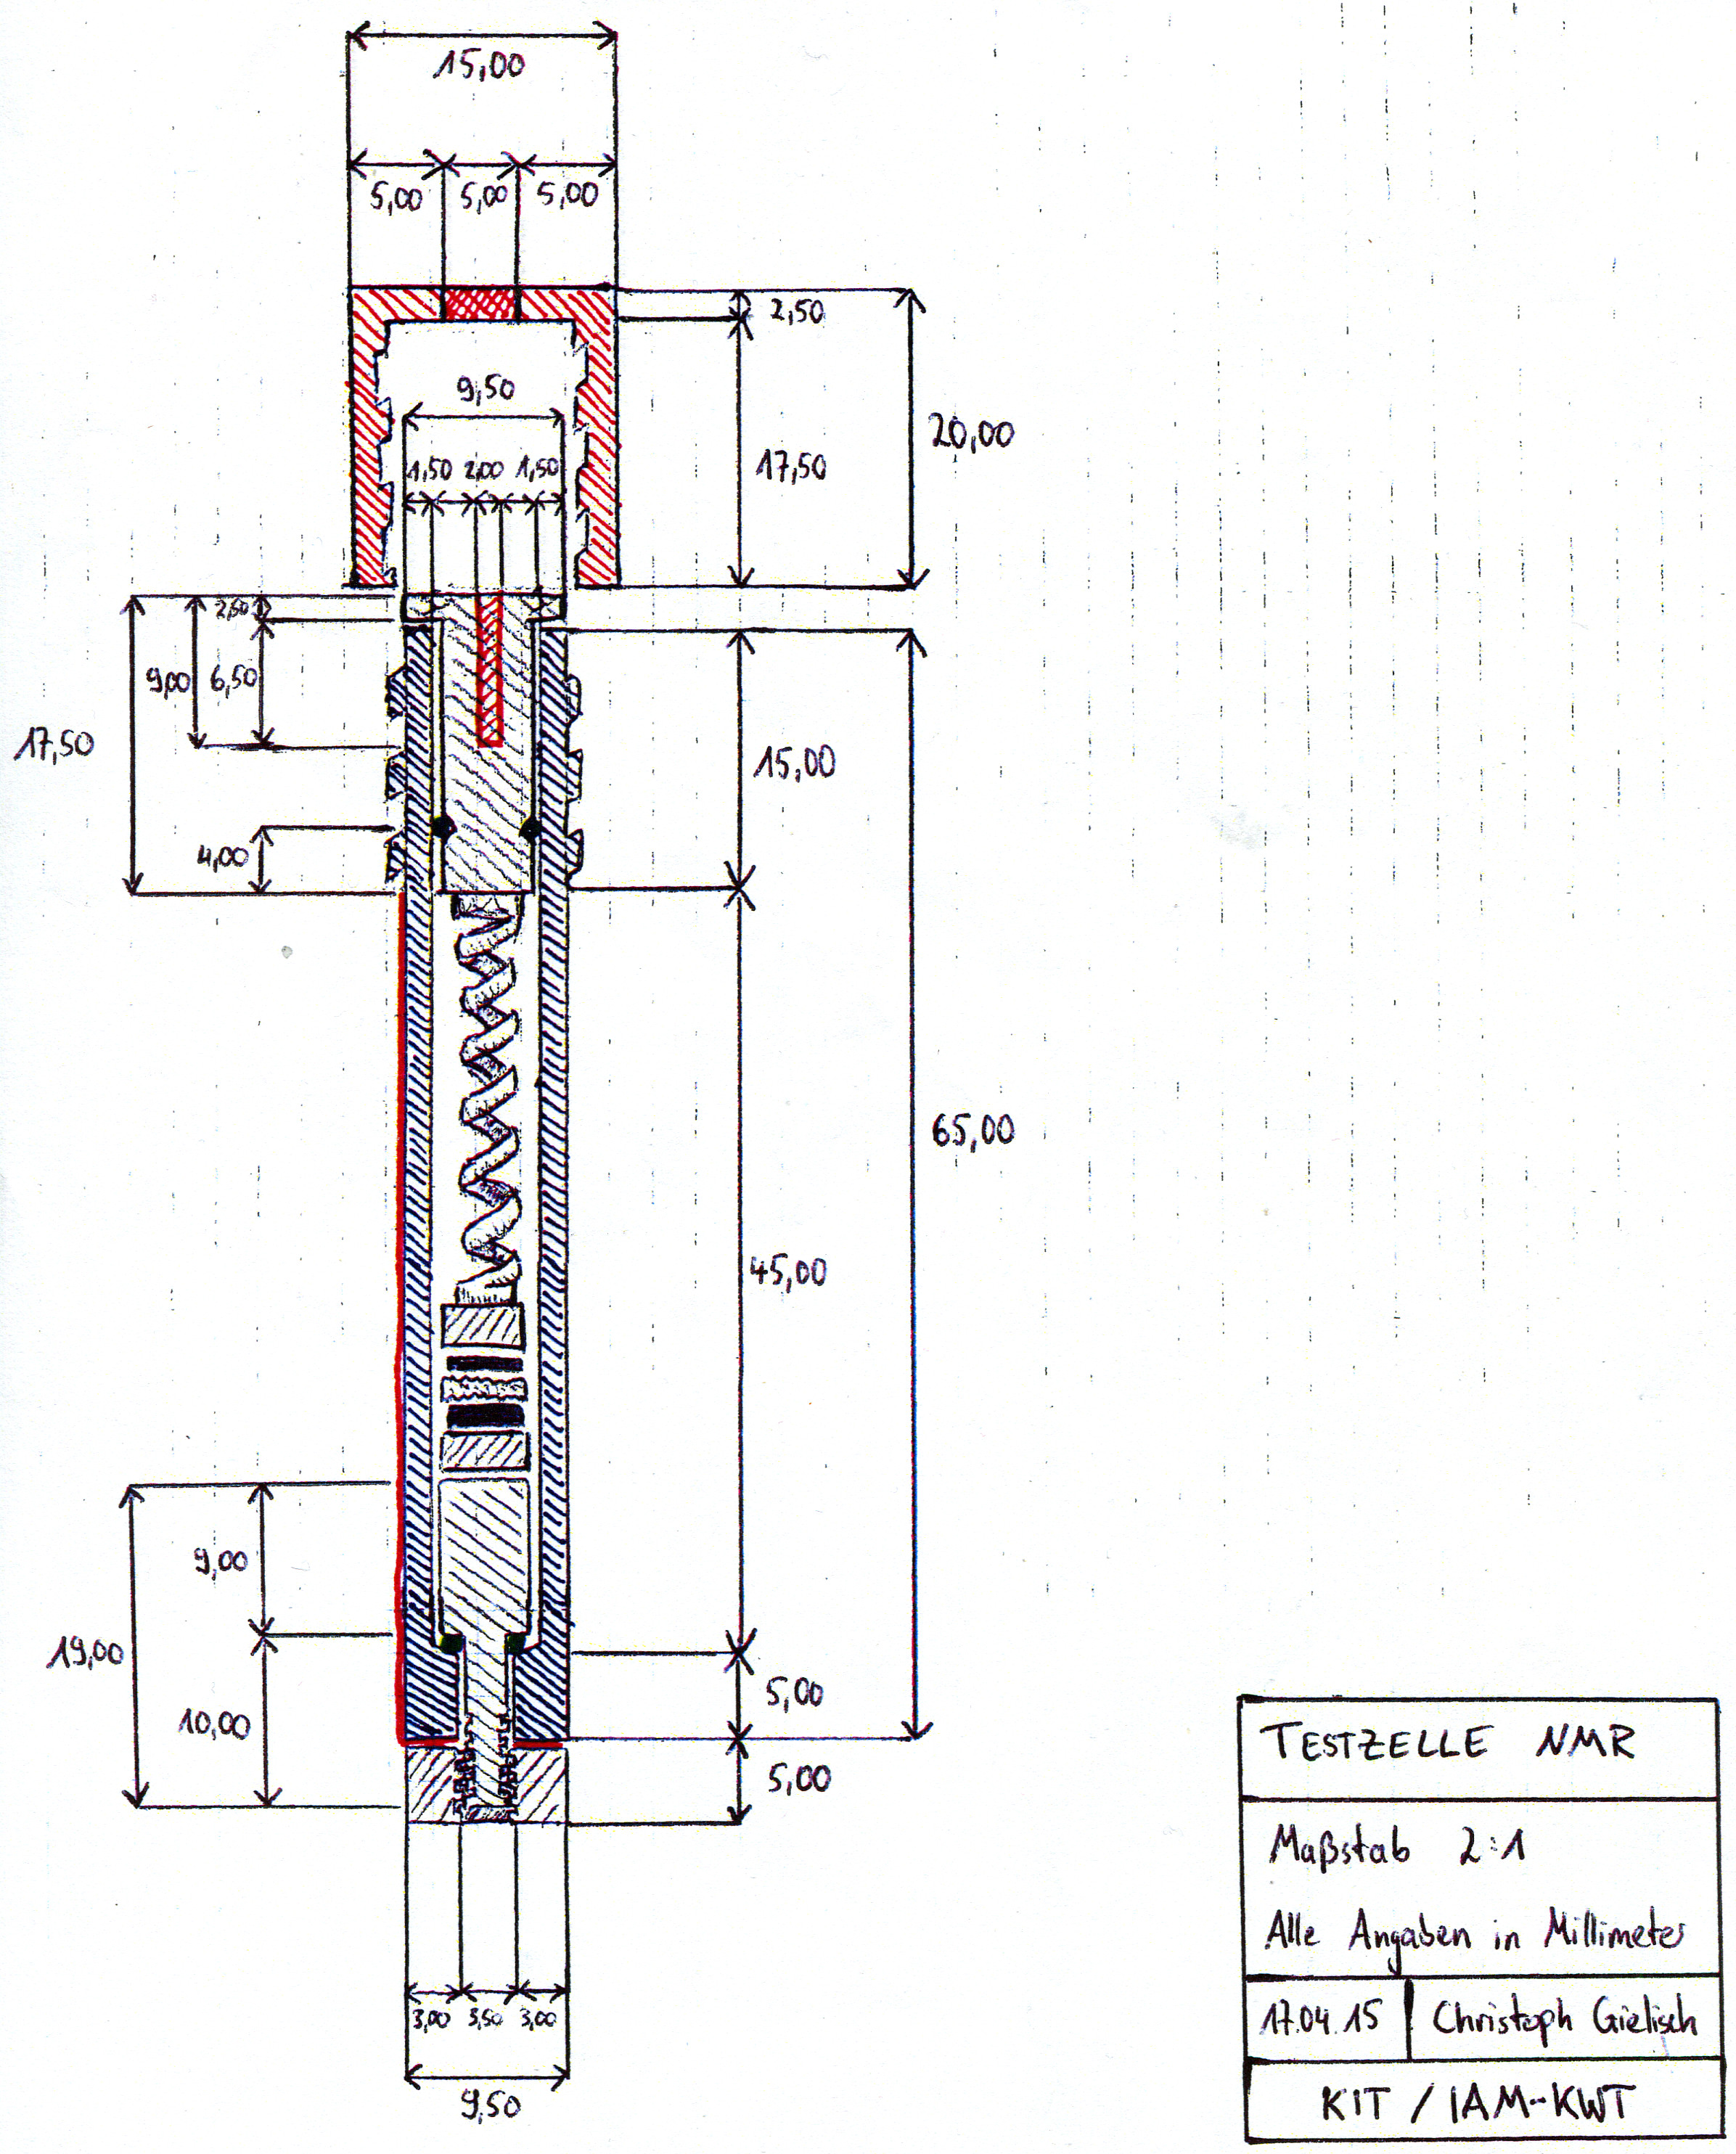
\includegraphics[width=1.0\columnwidth]{images/Skizze_Testzelle.jpg}
	\caption{Skizze der Testzelle}
	\label{skizze_testzelle}
\end{figure}
Der Aufbau des NMR-Spektrometers gibt eine zylindrische Form der einzuführenden Probe vor. Da die gewickelte Zellen für Festkörperelektrolytbatterien nicht geeignet sind, wird ein Knopfzellenaufbau gewählt. Für die einfachere Handhabung wird ein länglicheres Design mit einer normalen Druckfeder, ähnlich der bereits am IAM-KWT im Einsatz befindlichen Testzelle, umgesetzt. Jedoch musste der bisherige Abschluss der Zelle umgestaltet werden. Um in den Probenkopf eingeführt werden zu können, muss der Boden der neuen Zelle bündig mit der restlichen Zelle abschließen und darf nicht auskragen. Dies würde den optimalen Sitz der Spule verhindern. Der Verschluss kann daher nicht außenliegend erfolgen. Die Kontaktierung kann nicht nach unten hinweg erfolgen, weshalb an der Außenseite der Zelle nach oben hin eine Leitung existieren muss. Beide Maßnahmen erfordern ein neues Design des unteren Stempels sowie der äußeren Hülle. Der obere Stempel und die Feder müssen sowohl auf den kleineren Durchmesser hin angepasst werden, als auch aus amagnetischen Materialien gefertigt werden. Abbildung \ref{skizze_testzelle} zeigt skizzenhaft die Planung der neuen Testzelle.
\subsubsection{Die Glaszelle}
Als Material für die Zellhülle wurde Glas ausgewählt. Glas bietet den Vorteil einer optischen Kontrolle der Zelle während des manuellen Einbaus der verschiedenen Komponenten. Es ist auch bei dünnen Wandstärken ausreichend fest, womit der Innendurchmesser maximiert werden konnte. Glas ist ausreichend amagnetisch und kann gut bearbeitet werden.
\\\\
Die Glaszelle wurde von einem Glasbläser der Laborhandelsgesellschaft GmbH (Karlsruhe) aus einem Glasrohr gefertigt, welches unten nach innen verdickt und durchstochen worden ist und an das nach oben mit einem Standardgewindeteil (GL14) versehen worden ist.
\\\\
Die mitgelieferten Plastikdeckel mussten auf den maximalen Durchmesser der Kupferabschirmung von 16,5mm abgeschliffen werden. Dies erfolgte händisch auf einer Schleifmaschine des Typs DAP-V der Firma Struers.
\subsubsection{Die Stempel}
Die beiden Stempel wurden jeweils als CAD-Modell mit der Software Creo Parametric der Firma PTV geplant. Die Zeichnungen sind in Abbildung \ref{stempel_oben} und \ref{stempel_unten} dargestellt. Der obere Stempel entspricht dabei dem Stempel aus der existierenden Zelle mit angepasster Höhe, Durchmesser und Nut für den Dichtungsring. Die 2mm-Bohrung zur Kontaktierung bleibt erhalten. Der untere Stempel wurde komplett neu gestaltet. Er besteht aus einem Kopf mit einer Nut für den Dichtungsring, welcher für die Dichtigkeit der Zelle sorgt. Von ihm abgehend ist ein Stab mit einem M3-Isogewinde. Dieser passt durch die Aussparung der Glaszelle und ermöglicht das Befestigen des Stempels mit einer außenliegenden Mutter. Als Material kommt eine Messinglegierung zum Einsatz (\ce{CuZn39Pb3}), welche ausreichend amagnetisch (Suszeptibilität X $=\;-$0,173 · 10$^{-6}$ cm$^3$/g) ist. 
\\\\
Die Stempel wurden an einer CNC-Drehmaschine von Technikern der Technologiefabrik Karlsruhe gedreht. %Typ der Drehmaschine?
\begin{figure}
%mit Subfigures machen?
	\centering
	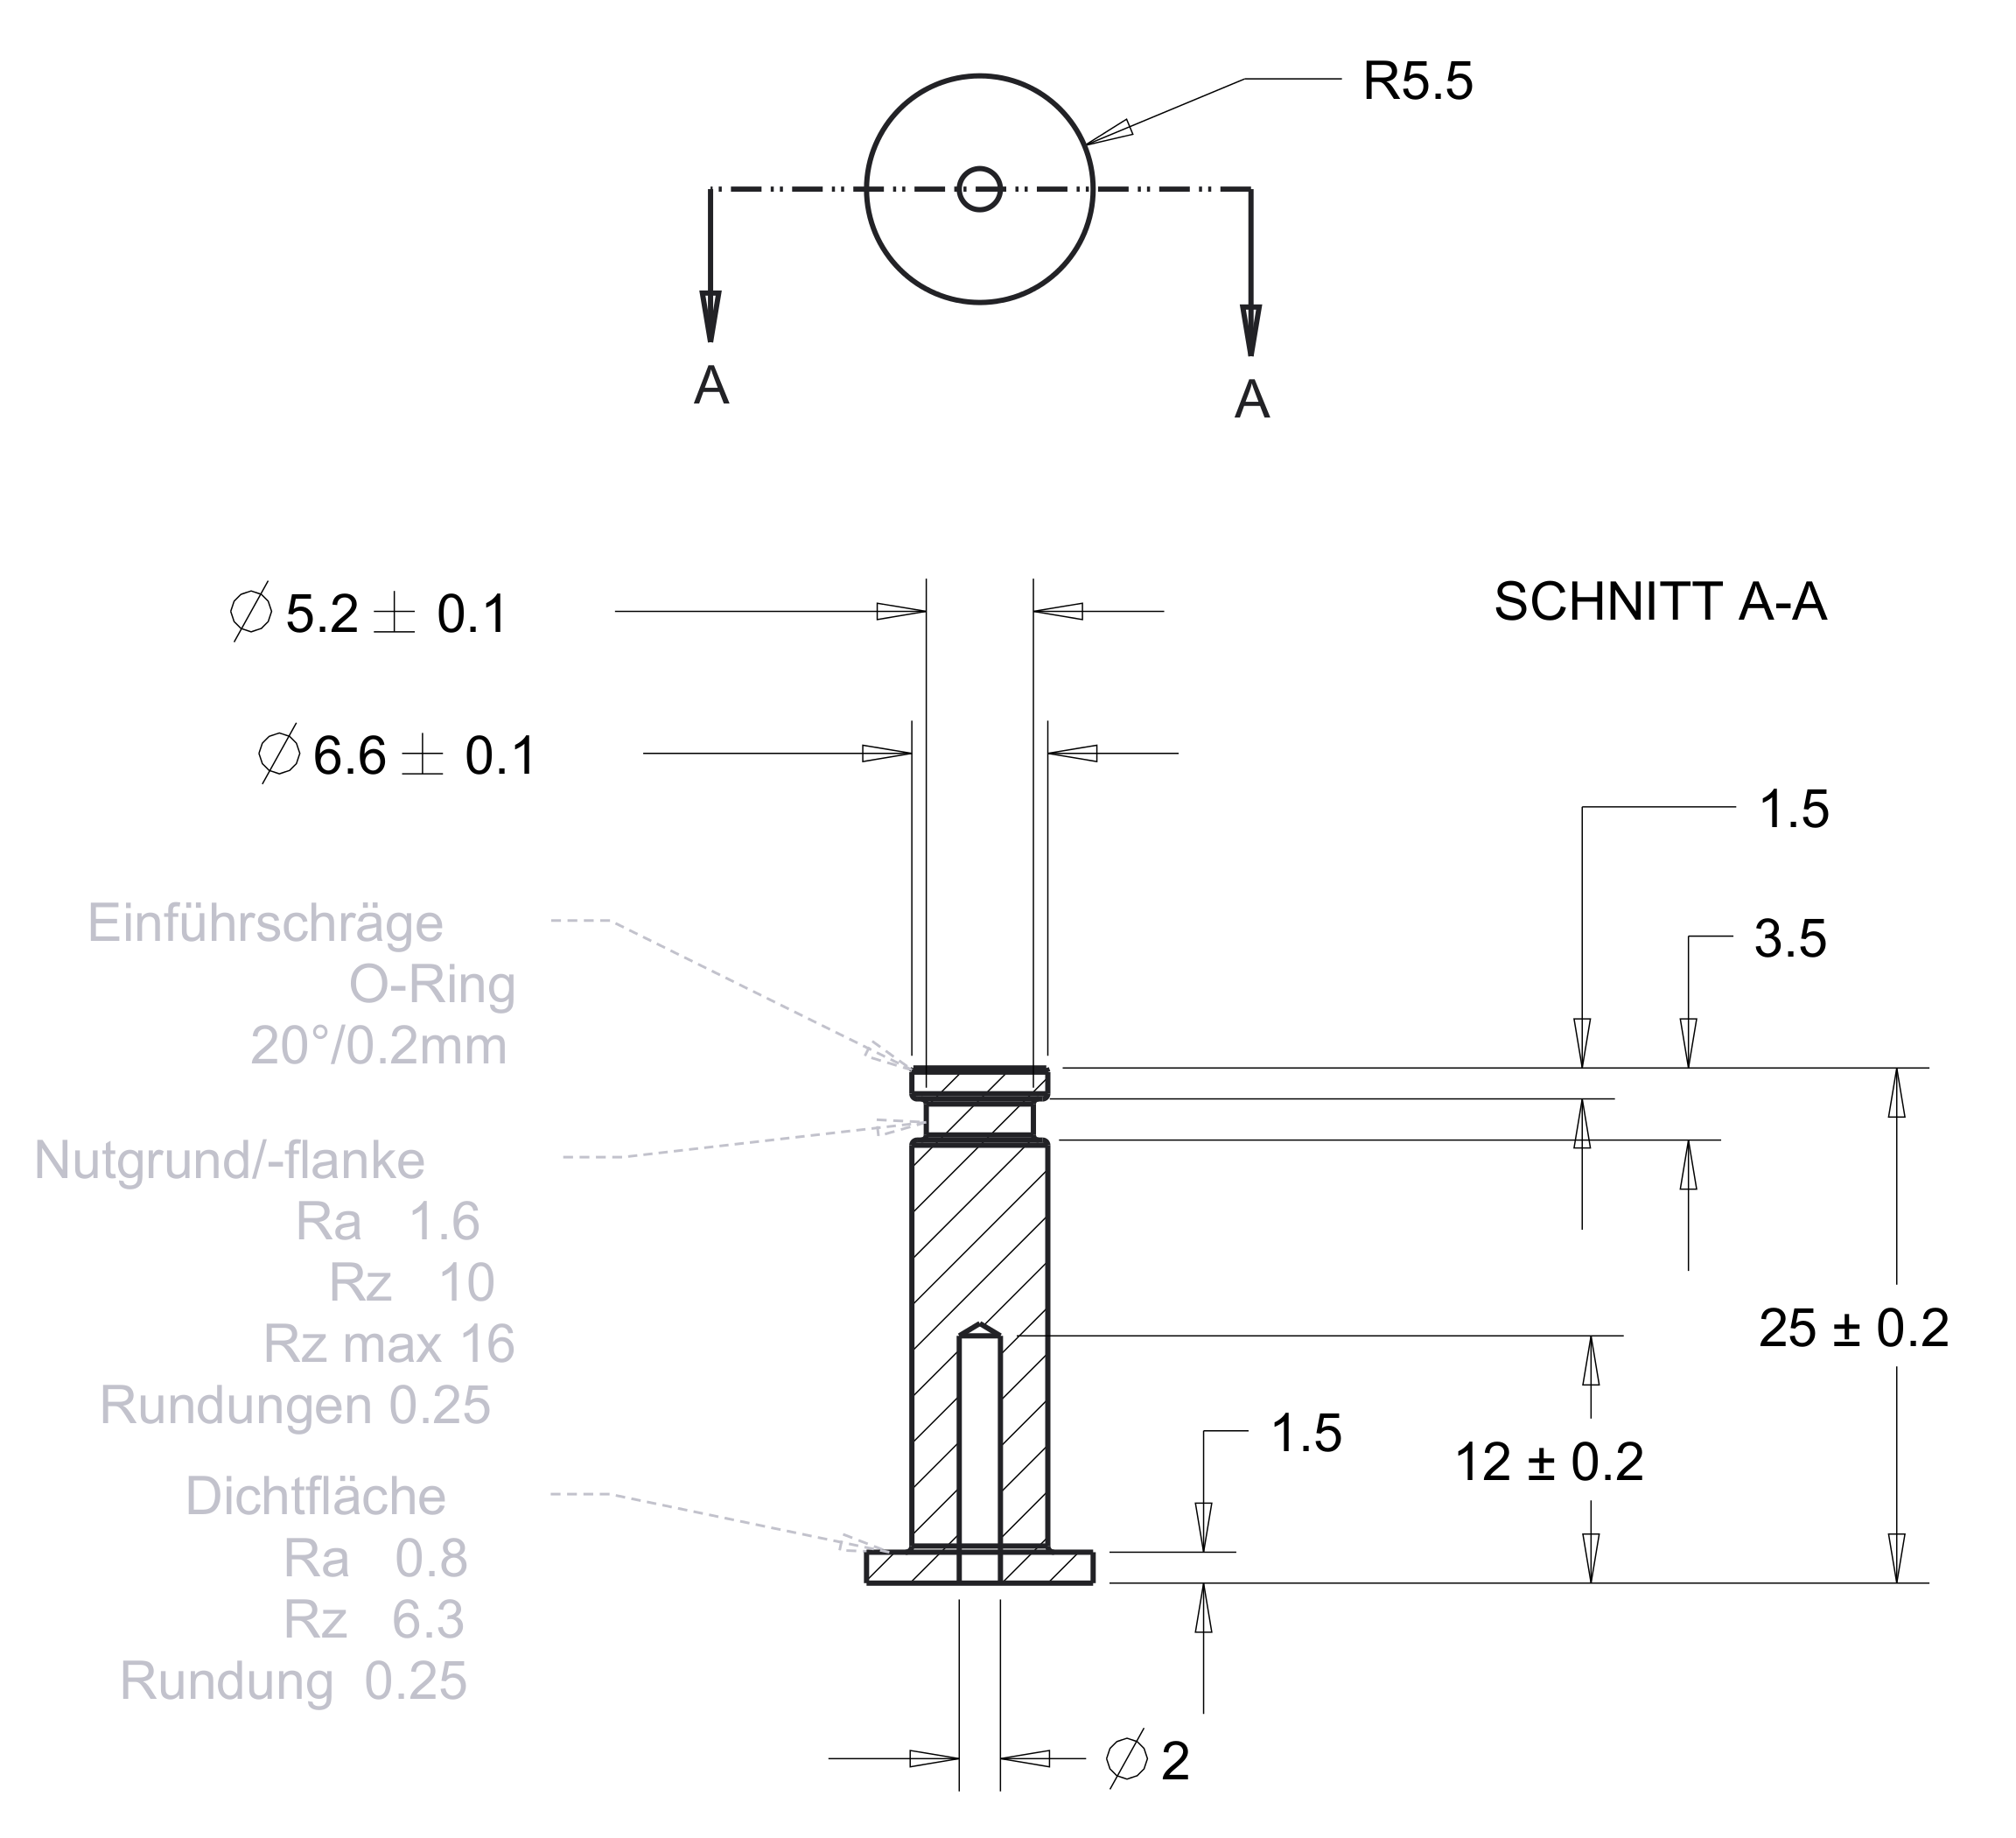
\includegraphics[width=0.7\columnwidth]{images/stempel_oben.png}
	\caption{Stempel oben}
	\label{stempel_oben}
\end{figure}
\begin{figure}
	\centering
	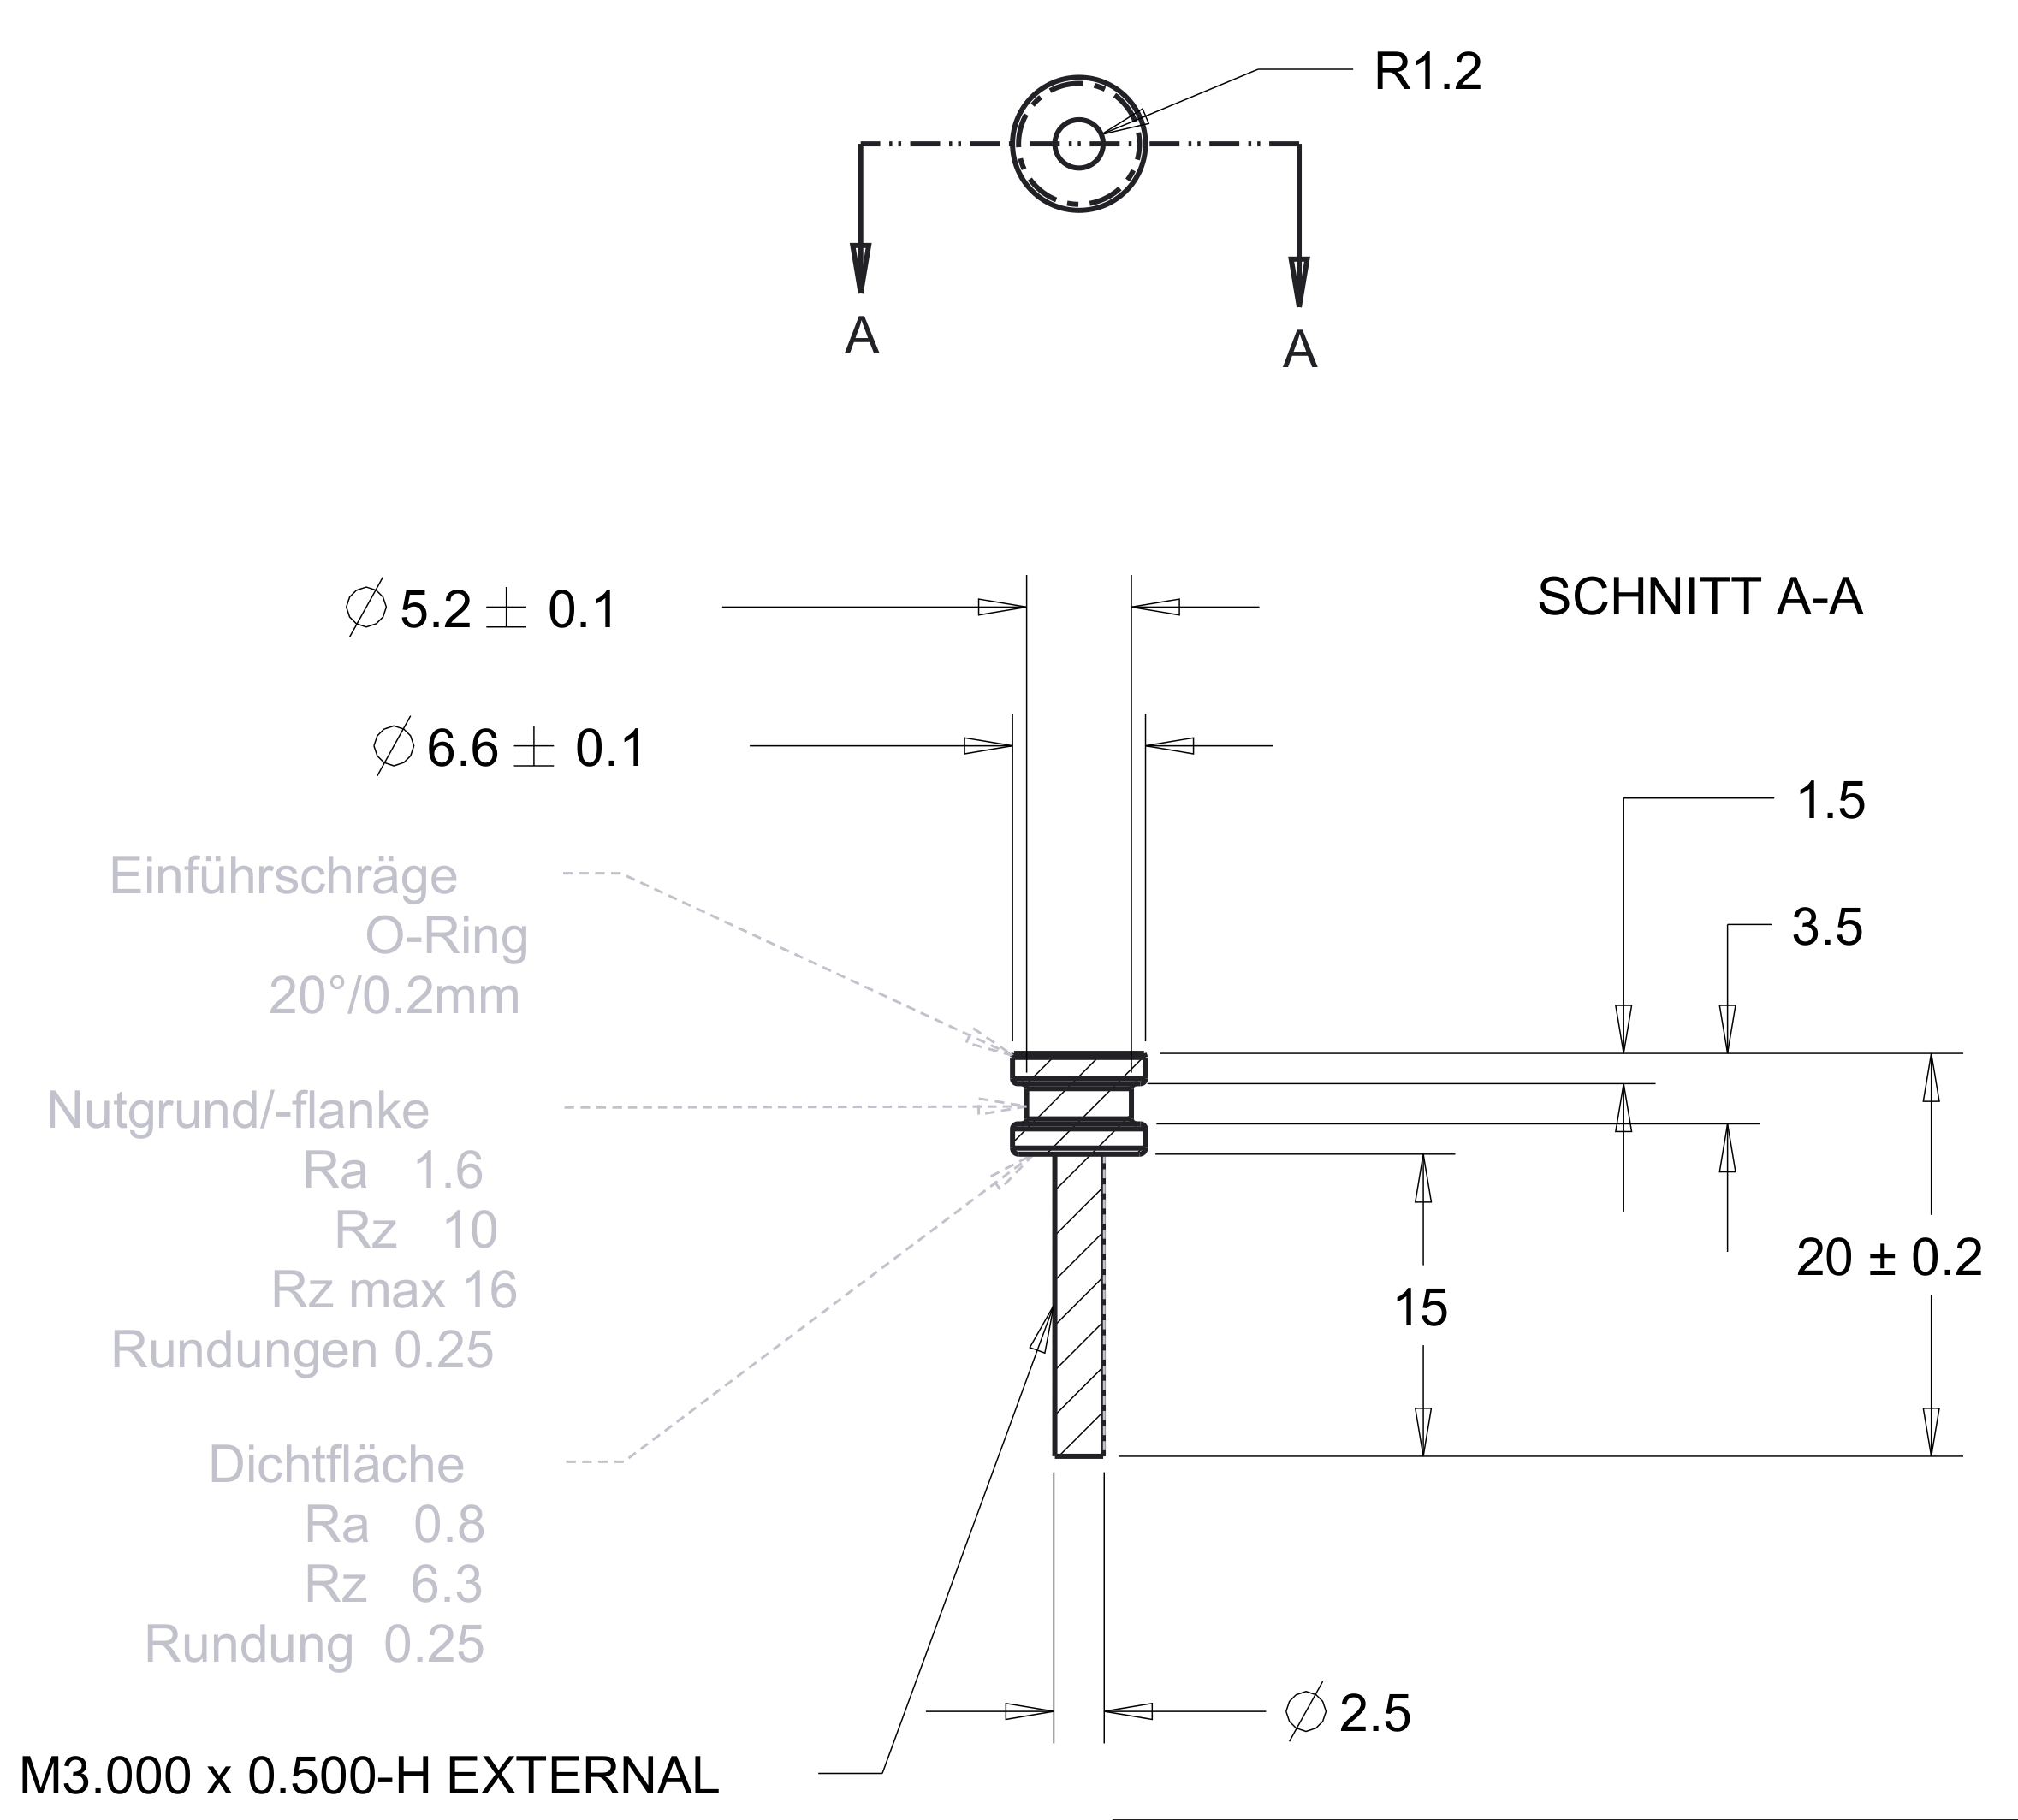
\includegraphics[width=0.7\columnwidth]{images/stempel_unten.png}
	\caption{Stempel unten}
	\label{stempel_unten}
\end{figure}
\begin{figure}
	\centering
	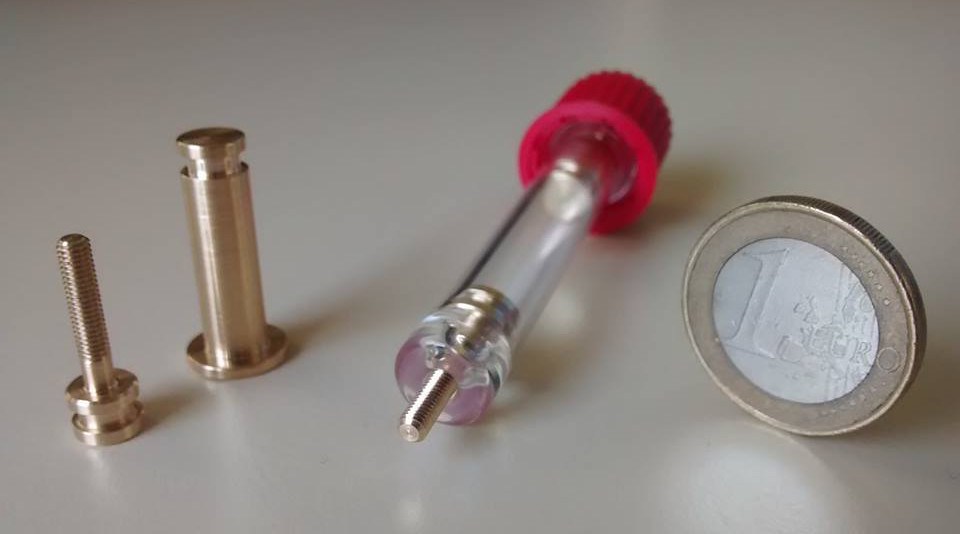
\includegraphics[width=1.0\columnwidth]{images/Stempel_Foto_cutted.jpg}
	\caption{Übersicht über die verschiedenen Teile des in-situ-Testzelle (besseres Foto machen!)}
	\label{stempel_foto}
\end{figure}
\subsubsection{Die Mutter}
Durch den Einsatz des M3-Standardgewindes bei den Stempeln, konnte bei der Mutter ein Standardmodell aus Messing aus dem Fachhandel eingesetzt werden.
\subsubsection{Die Feder}
Die Feder stellte besondere Herausforderungen an die Materialauswahl. So musste neben der amagnetischen Eigenschaft auch eine gute elastische Verformbarkeit und eine gute Leitfähigkeit für den elektrischen Strom gegeben sein. Neben Messing wurde daher auch Federbronze (\ce{CuSn6}) und Kupferberyllium (\ce{CuBe2}) als mögliche Materialien betrachtet.
% Tabelle mit Übersicht?
\\\\
Die Feder wird dabei so ausgelegt, dass der Anpressdruck auf die Zelle möglichst gleich ist, wie bei der bereits am IAM-KWT existierenden Zelle. Diese baut bei einem Federweg von 25 mm und einer Federrate von 0,541 N/mm eine Kraft von 13,525 N auf. Bei einer Fläche von 93,3 mm$^2$ entspricht dies einem Anpressdruck von 0,145 N/mm$^2$. Die Höhe der neuen Feder wurde auf 30 mm festgelegt, der zu absolvierende Federweg bei Einbau beträgt 10 mm. Die Fläche auf der die Kraft aufgebracht wird beträgt 36,32 mm$^2$. Um den gleichen Anpressdruck zu gewährleisten, benötigt die neue Feder daher eine Kraft von 5,266 N, was einer Federrate von 0,527 N/mm entspricht.
\\\\
Die Feder wurde von Febrotec Federn (Halver) aus Kupferberyllium gefertigt. Der Drahtdurchmesser beträgt 0,75 mm, der Federnaußendurchmesser 6,5 mm. Ungespannt hat die Feder eine Höhe von 30mm. %Windungszahl?
\subsubsection{Die Positionsplättchen}
Die Positionsplättchen sorgen dafür, dass sich die eigentliche Batteriezelle, also die Elektroden und der Elektrolyt, im sensitiven Bereich der Spule befindet. Da sie sich selbst dadurch unmittelbar im Messbereich aufhalten, wird auf eine vollständige Metallfertigung verzichtet, um die dämpfende Wirkung zu minimieren. Stattdessen werden von einem Teflonstab passende Scheiben abgeschnitten und plan geschliffen. Anschließend werden die beiden Grundflächen mit Kupferklebeband abgeklebt. Die beiden Seiten sind über einen dünnen Kupferstreifen an der Seite miteinander verbunden. 
\section{Bau und Betrieb der Batterie-Testzellen}
\begin{figure}
	\centering
	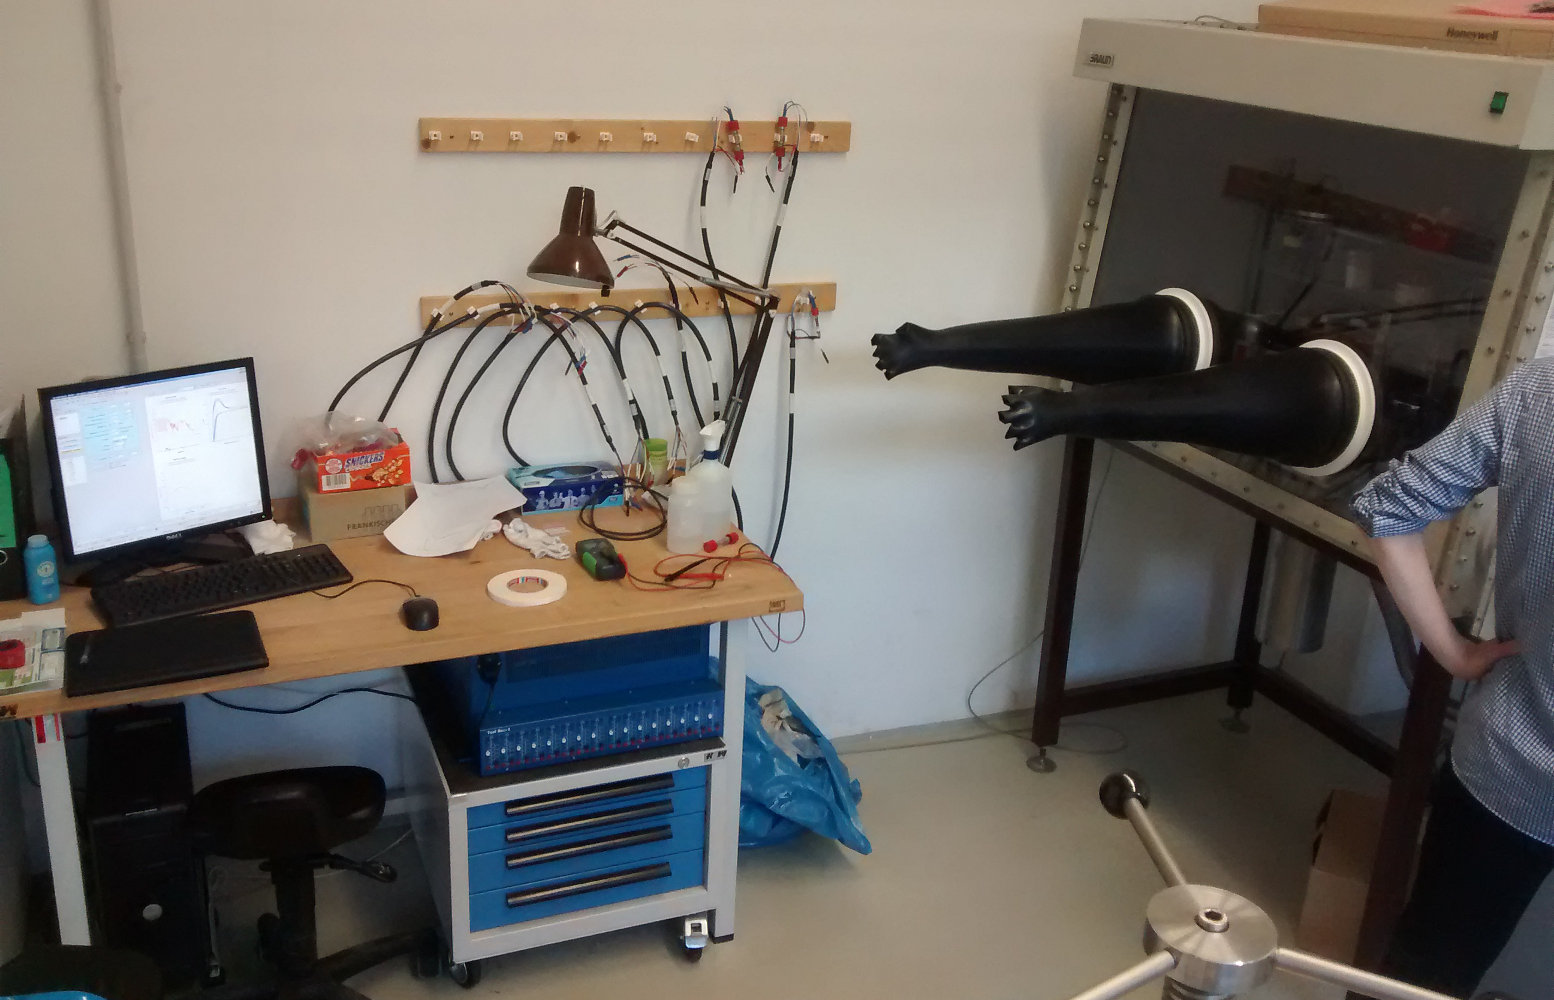
\includegraphics[width=0.95\columnwidth]{images/Messplatz.jpg}
	\caption{Messplatz für Batteriezellen mit Handschuhbox zum Bau (rechts), Ansteuerungselektronik und Aufbewahrung (mitte) sowie Kontrolle und Aufzeichnung durch Computer (links). --> Besseres Foto}
	\label{messaufbau}
\end{figure}
Zunächst werden aus den gegossenen Elektrodenfolien Proben entnommen. Dies geschieht händisch mit einem 6mm-Stanzeisen. Die Proben werden anschließend in eine Handschuhbox der Firma mBraun eingeschleust. Der Zusammenbau der Testzellen erfolgt dort unter Argonatmosphäre. Die Proben werden dabei jeweils als Kathode verbaut. Als Anode kommt Lithiummetall (99,9\%, Aldrich) zum Einsatz. Von diesem wird die äußerste Schicht abgetragen, um mögliche passivierte Stellen zu entfernen. Anschließend wird das Lithium mit einer Handwalze auf einen halben Minimeter gewalzt, wodurch seine Oberfläche geglättet wird. Danach kann mit einem 6mm-Stanzeisen die Lithium-Elektrode hergestellt werden.
\\\\
Der Zusammenbau besteht aus dem Einsetzen des unteren Stempels sowie eines Positionsplättchens in die Zelle. Darauf wird zunächst die Kathodenprobe gelegt und mit zwei Separatoren abgedeckt. Durch die zweifache Bedeckung führt ein Defekt eines Separators nicht zum Ausfall der Zelle. Die Separatoren werden mit 25$\mu$l Elektrolyt benetzt. Auf die Separatoren wird die Lithium-Anode und ein weiteres Positionsplättchen gelegt. Um einen Anpressdruck der Teile zu gewährleisten wird nun die Feder eingebaut und die Zelle mit dem oberen Stempel verschlossen. Beide Stempel können nun mit Mutter und Deckel fixiert werden. Danach kann die Zelle ausgeschleust und an das Messsystem angeschlossen werden.
% Was genau ist der Separator, was genau der Schwefel-Elektrolyt
\\\\
Die Batteriezellen werden mit dem Messsystem VMP3 der Firma BioLogic untersucht. Dieses wird mit der Software ECLab in der Version 10.33 angesteuert und ermöglicht die Zyklierung der Zellen, zyklische Voltametrie sowie Impedanzmessungen. Die aufgezeichneten Daten können als zView-Datei exportiert und weiterverarbeitet werden.
% ECLab-Programme?
\chapter{Ergebnisse}
Die angefertigten Pulver werden mittels Röntgendiffraktion und MAS-NMR untersucht. Für die aus ihnen hergestellten Batterieproben werden Ladekennlinien erstellt. Außerdem werden sie mittels zyklischer Voltametrie und Impedanzmessungen analysiert. Die Funktionalität der in-situ-Testzelle wird mit einer Lithium-Schwefel-Zelle gezeigt.
\section{Pulveranalyse}
\subsection{LATP}
\subsubsection{XRD-Analyse}
\subsubsection{MAS-NMR-Analyse}
\begin{figure}
	\centering
	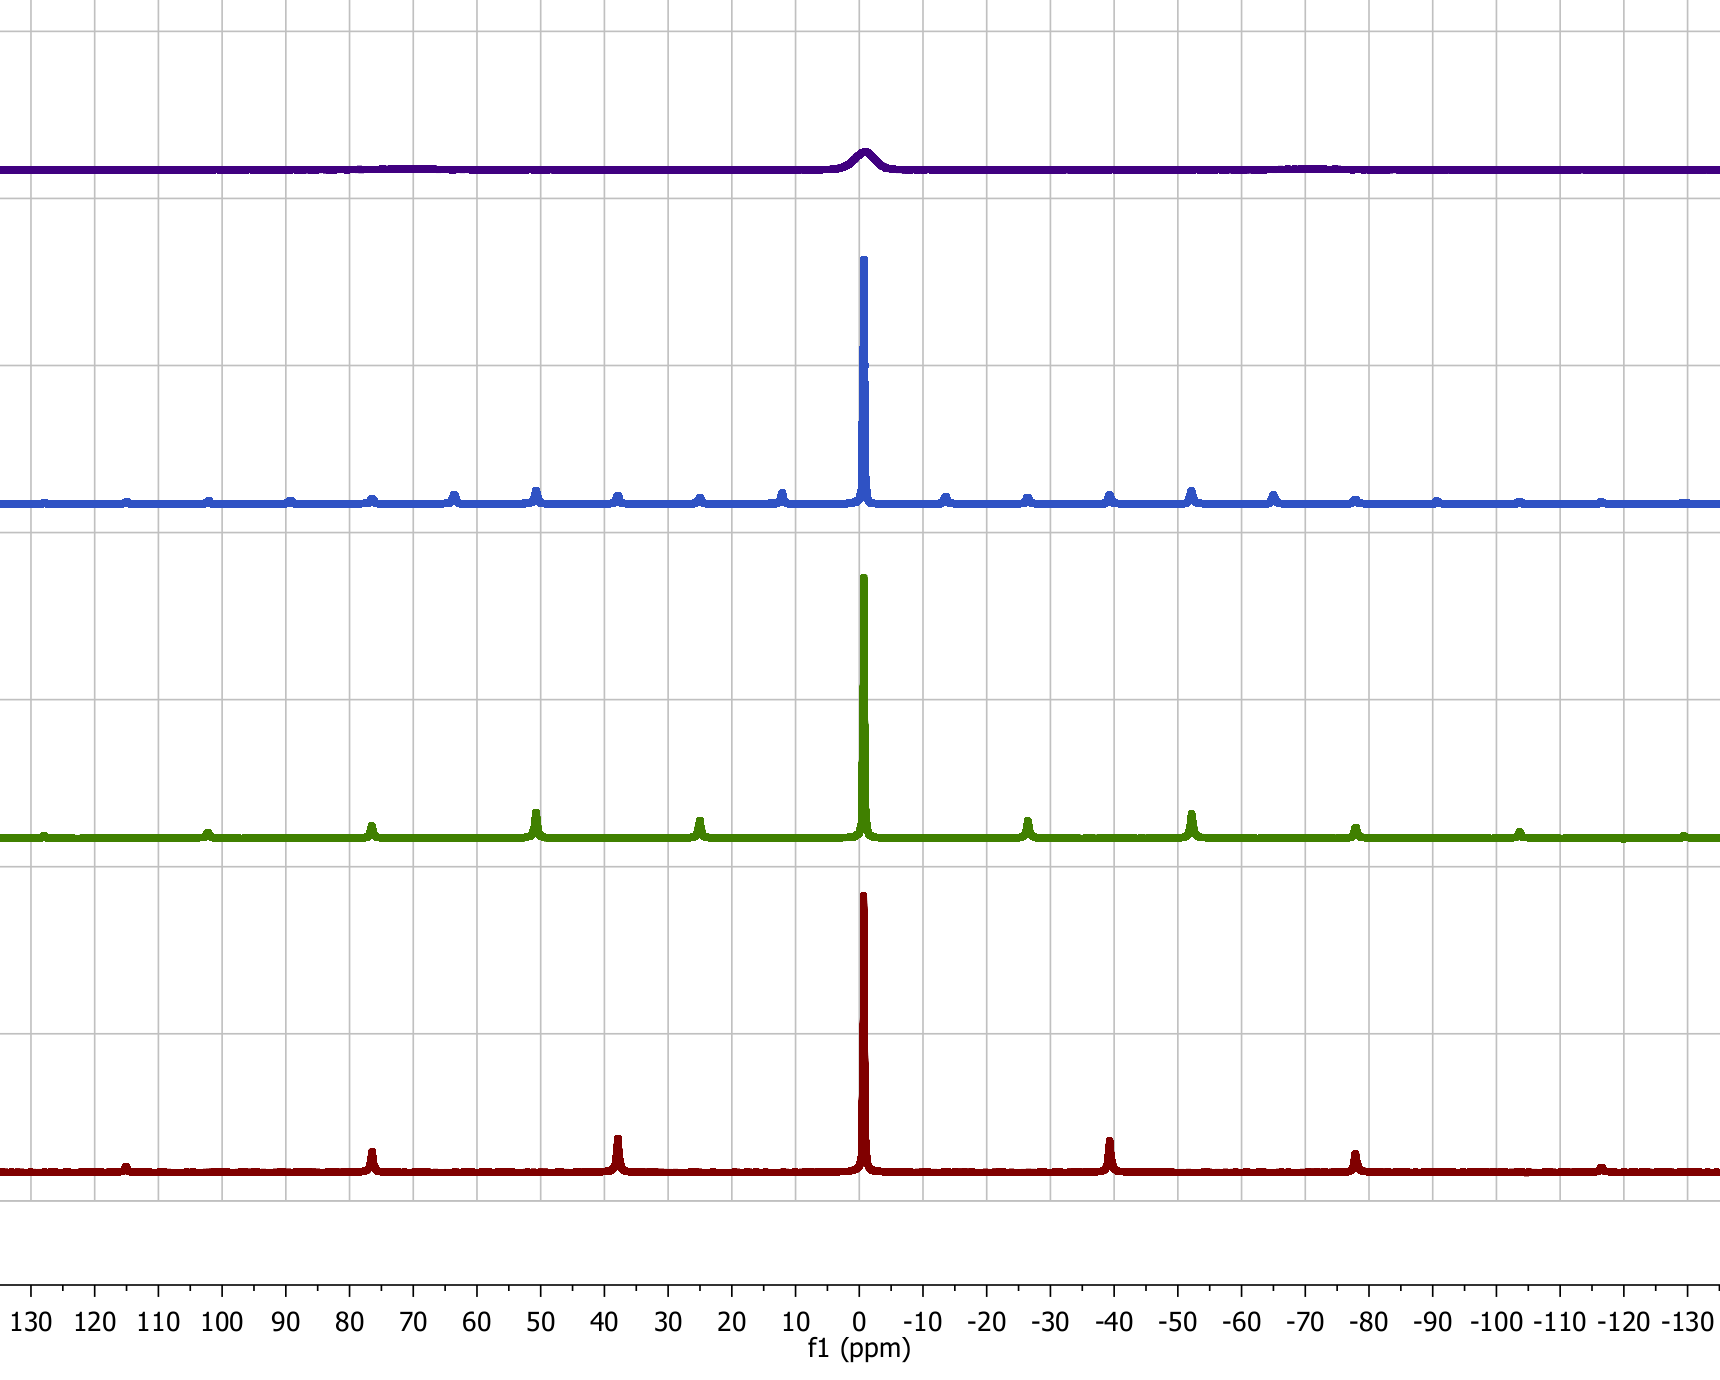
\includegraphics[width=1.0\columnwidth]{images/Spektrum_LATP.png}
	\caption{MAS-NMR-Spektrum von LATP bei verschiedenen Umdrehungsgeschwindigkeiten (lila 0kHz, blau 2kHz, grün 4kHz, rot 6kHz)}
	\label{nmr_mas_LATP}
\end{figure}
\subsection{\ce{LiTiPO5}}
\subsubsection{XRD-Analyse}
\subsubsection{MAS-NMR-Analyse}
\subsection{Weitere Pulver}
Die bereits am Institut vorhandenen Pulver wurden bereits mittels Röntendiffraktometrie charakterisiert. Die zugrundeliegenden Daten werden in Kapitel \ref{methodik_weitere_Pulver} dargestellt. Daher wurde für diese Gruppe Pulver lediglich die MAS-NMR zur weiteren Charakterisierung angewandt.
\subsubsection{LAGP}
\subsubsection{LTO}
\subsubsection{LLTO}
\subsubsection{LiCl}
\begin{figure}
	\centering
	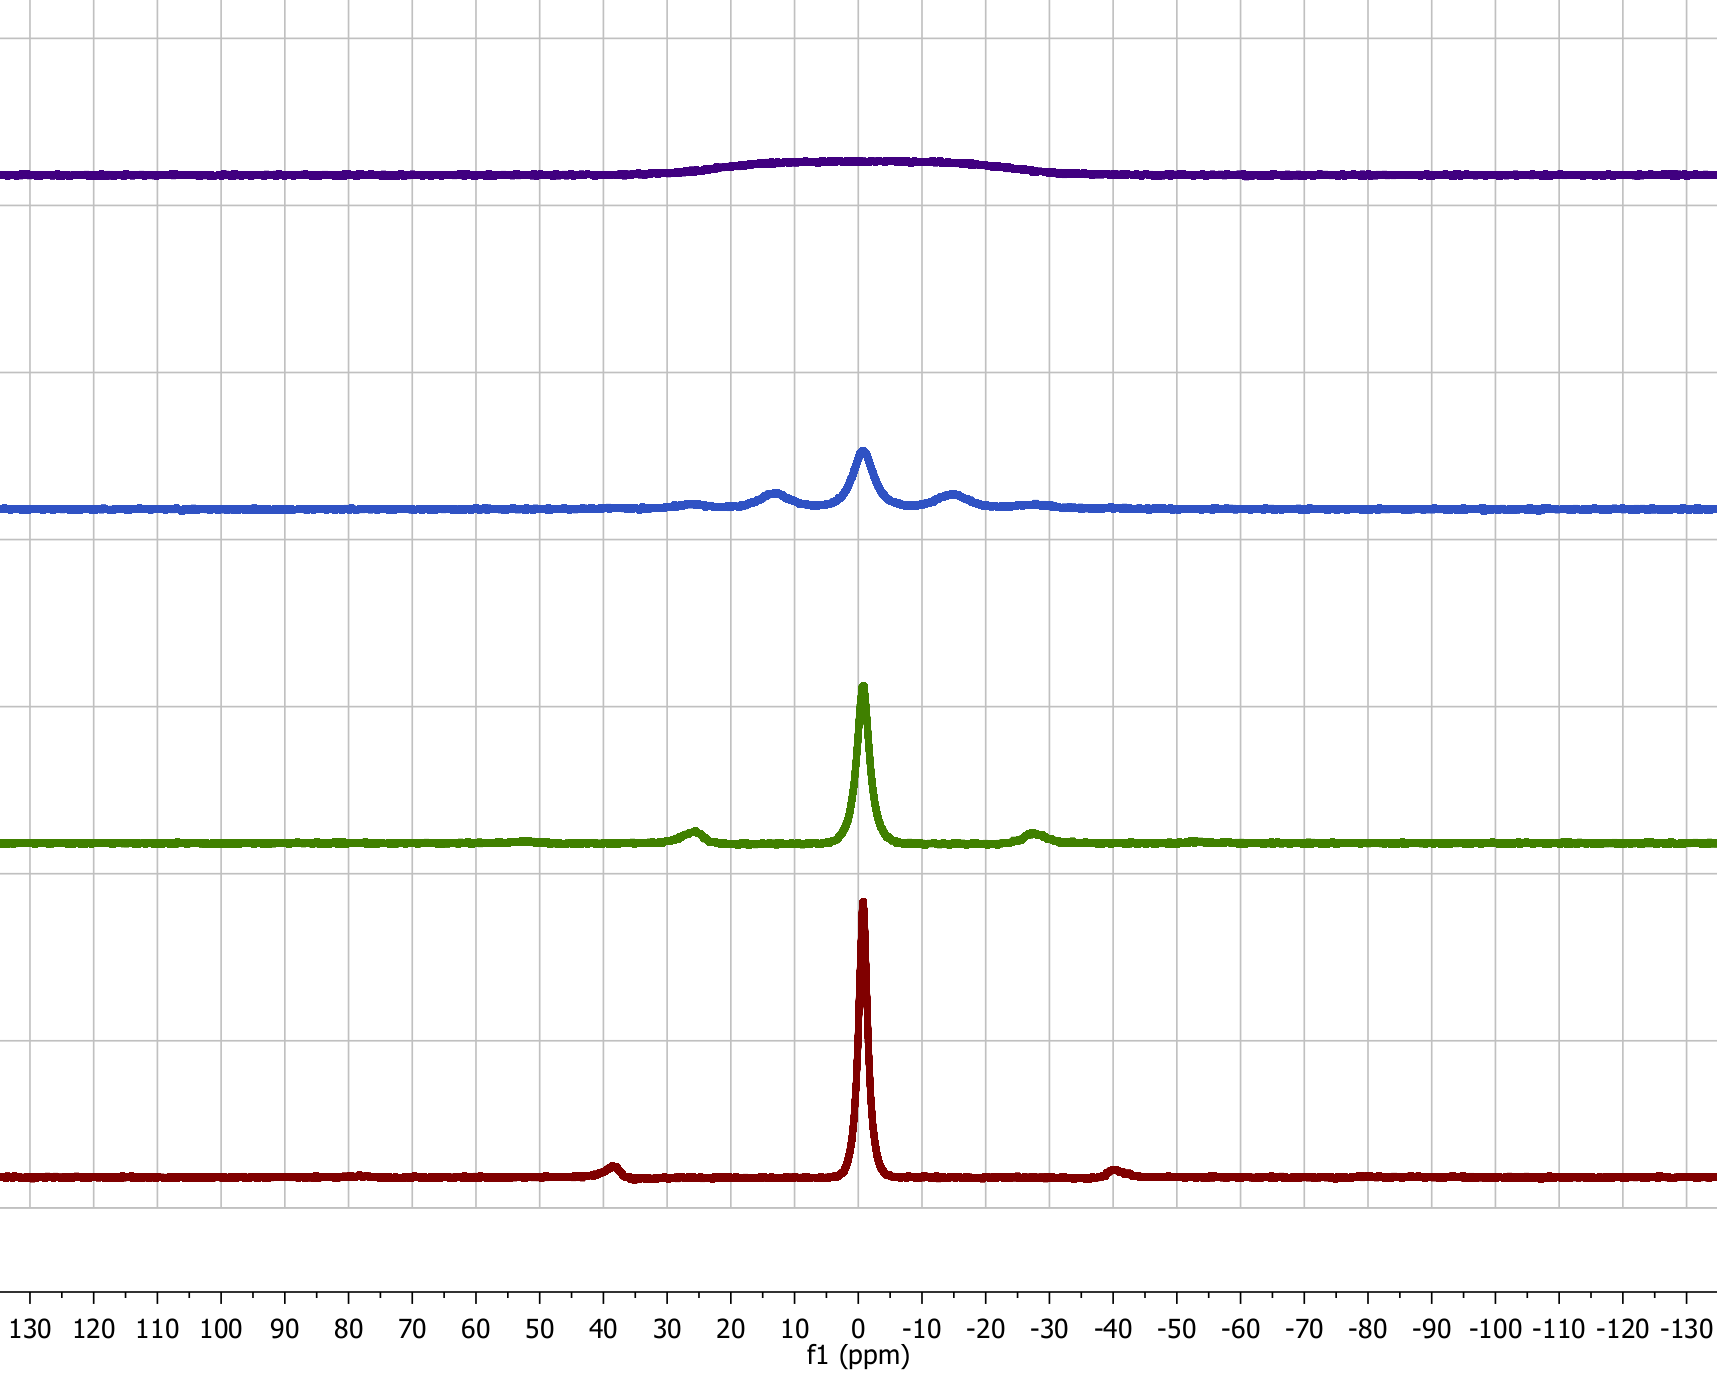
\includegraphics[width=1.0\columnwidth]{images/Spektrum_LiCl.png}
	\caption{MAS-NMR-Spektrum von LiCl bei verschiedenen Umdrehungsgeschwindigkeiten (lila 0kHz, blau 2kHz, grün 4kHz, rot 6kHz)}
	\label{nmr_mas_LiCl}
\end{figure}
\section{Batterietests}
\subsection{\ce{LiCoO2}}
\subsubsection{Zyklische Voltametrie}
\subsubsection{Ladekennlinien}
\subsubsection{Impedanzmessungen}
\subsection{Schwefel}
\subsubsection{Zyklische Voltametrie}
\subsubsection{Ladekennlinien}
\subsubsection{Impedanzmessungen}
\subsection{LATP}
\subsubsection{Zyklische Voltametrie}
\subsubsection{Ladekennlinien}
\subsubsection{Impedanzmessungen}
\subsection{LAGP}
\subsubsection{Zyklische Voltametrie}
\subsubsection{Ladekennlinien}
\subsubsection{Impedanzmessungen}
\subsection{LTO}
.
\subsubsection{Zyklische Voltametrie}
\subsubsection{Ladekennlinien}
\subsubsection{Impedanzmessungen}
\subsection{LLTO}
\subsubsection{Zyklische Voltametrie}
\subsubsection{Ladekennlinien}
\subsubsection{Impedanzmessungen}
\subsection{LTO-LLTO-Gefüge}
\subsubsection{Zyklische Voltametrie}
\subsubsection{Ladekennlinien}
\subsubsection{Impedanzmessungen}
\section{NMR-Messungen}
\subsection{Referenzmessung}
\subsection{Lithium-Schwefel-Zelle}
\chapter{Diskussion}
\section{Anwendbarkeit NMR}
\section{Vergleich Batterien}
\chapter{Fazit}
\section{Zusammenfassung}
\section{Ausblick}
% der Anhang
\renewcommand{\thesection}{\Alph{section}}
%\appendix
%\addchap{Anhang}
%\section{Parametereinstellungen}
%\section{Vergleichsbilder}

% das Abbildungsverzeichnis
\cleardoublepage
% \phantomsection
\addcontentsline{toc}{chapter}{Abbildungsverzeichnis}
\listoffigures

 % das Literaturverzeichnis
\cleardoublepage
% \phantomsection
\addcontentsline{toc}{chapter}{Literaturverzeichnis}
\bibliographystyle{unsrtdin}
\bibliography{literatur} 

% das ist wohl jetzt das Ende des Dokumentes
\end{document}